% Documento de prueba: compila solo las secciones 4-7.
% En el informe real, copie el preámbulo que falte y ponga %% =====================================================================
%% GenVar-PE · Hito 2 · Secciones 4 a 7
%% Generado por tex/construir_tex.py a partir de sql/*.sql y exp/resultados.json
%% =====================================================================

\section{Implementación de la base de datos}

La base de datos se implementó en PostgreSQL 16~\cite{postgres} dentro del esquema \texttt{genvar}. Todo el código está
en la carpeta \texttt{sql/} del repositorio del proyecto y se ejecuta en este orden:

\begin{table}[H]
\centering\small
\begin{tabular}{@{}ll@{}}
\toprule
Archivo & Contenido \\
\midrule
\texttt{01\_\allowbreak{}esquema.sql} & Creación de tablas, llaves y restricciones (4.1) \\
\texttt{02\_\allowbreak{}vistas.sql} & Vistas de usuario (4.4) \\
\texttt{03\_\allowbreak{}procedimientos.sql} & Procedimientos almacenados y funciones (4.5) \\
\texttt{04\_\allowbreak{}triggers.sql} & Triggers (4.6) \\
\texttt{05\_\allowbreak{}roles.sql} & Roles y permisos por tipo de usuario \\
\texttt{06\_\allowbreak{}generar\_\allowbreak{}datos.sql} & Simulación de datos para los cuatro escenarios (4.3) \\
\texttt{07\_\allowbreak{}consultas.sql} & Las consultas C1--C8 (5.1.2) \\
\texttt{08\_\allowbreak{}indices.sql} & Planes de índices evaluados e índices finales (5.3) \\
\texttt{09\_\allowbreak{}pruebas.sql} & Pruebas de triggers y procedimientos (4.6) \\
\bottomrule
\end{tabular}
\caption{Scripts de la implementación.}
\end{table}

\subsection{Creación de tablas}\label{sec:creacion}

Las tablas siguen al pie de la letra el modelo relacional y el diccionario de datos de la Sección~3.
Cada regla semántica que se puede expresar dentro de una sola tabla se implementó como restricción
declarativa (\texttt{PRIMARY KEY}, \texttt{UNIQUE}, \texttt{FOREIGN KEY}, \texttt{NOT NULL} y \texttt{CHECK});
las que necesitan mirar otra tabla se implementaron con triggers (Sección~4.6). Las decisiones más
importantes son:

\begin{itemize}
  \item \textbf{RS19 con una llave foránea compuesta.} \texttt{genotipo(id\_\allowbreak{}muestra, id\_\allowbreak{}corrida)} referencia a
        \texttt{muestra\_\allowbreak{}corrida}, no a \texttt{muestra} y \texttt{corrida} por separado. Así es imposible guardar
        un genotipo de una muestra en una corrida en la que no fue secuenciada, sin escribir un trigger.
  \item \textbf{Especialización Is-A (RS3) con una tabla por clase.} \texttt{muestra\_\allowbreak{}germinal} y
        \texttt{muestra\_\allowbreak{}tumoral} tienen como llave primaria y foránea a \texttt{id\_\allowbreak{}muestra}. Que sea disjunta y
        total no lo puede garantizar un \texttt{CHECK}, por eso lo hacen los triggers T4 y T5.
  \item \textbf{Entidad débil \texttt{exon}.} Su llave es \texttt{(id\_\allowbreak{}gen, numero\_\allowbreak{}exon)} y se borra en cascada con su gen.
  \item \textbf{Llave natural de la variante (RS13).} Se usa la llave sustituta \texttt{id\_\allowbreak{}variante BIGSERIAL} para que
        \texttt{genotipo} sea liviana, y la llave natural \texttt{(id\_\allowbreak{}cromosoma, posicion, alelo\_\allowbreak{}ref, alelo\_\allowbreak{}alt)}
        queda como \texttt{UNIQUE}.
  \item \textbf{Atributo derivado.} \texttt{tipo\_\allowbreak{}variante} (RS15) no se guarda; se calcula en la vista \texttt{v\_\allowbreak{}variante}
        para no romper la FNBC.
  \item \textbf{Borrado en cascada (RS23).} \texttt{muestra}, \texttt{muestra\_\allowbreak{}corrida} y \texttt{genotipo} usan
        \texttt{ON DELETE CASCADE} hacia su padre.
  \item \textbf{Corrección al diccionario.} Al implementar se detectó que \texttt{secuenciador.tecnologia} no cabía en
        \texttt{VARCHAR(12)}, porque el valor \texttt{'LECTURA\_\allowbreak{}CORTA'} tiene 13 caracteres. Se cambió a \texttt{VARCHAR(14)}
        y el diccionario de datos de la Sección~3 ya refleja el cambio.
\end{itemize}

Además se agregaron tres tablas que el Hito~1 necesitaba pero no había modelado como tablas:
\texttt{informe} (fecha del último informe de cada donante, usada por la consulta C8),
\texttt{anotacion\_\allowbreak{}historial} (reclasificaciones de ClinVar, la llena el trigger T8) y
\texttt{bitacora} (auditoría de cargas y revocaciones). El Listado~\ref{lst:genotipo} muestra la tabla de hechos.
\begin{lstlisting}[language=SQL,caption={Tablas \texttt{muestra\_corrida} y \texttt{genotipo} (extracto de \texttt{01\_esquema.sql})},label=lst:genotipo]
CREATE TABLE muestra_corrida (
    id_muestra       VARCHAR(14)  REFERENCES muestra ON DELETE CASCADE,
    id_corrida       VARCHAR(30)  REFERENCES corrida,
    barcode          VARCHAR(20)  NOT NULL,
    lecturas_totales BIGINT       CHECK (lecturas_totales >= 0),
    cobertura_media  NUMERIC(7,2) CHECK (cobertura_media >= 0),
    pct_q30          NUMERIC(5,2) CHECK (pct_q30 BETWEEN 0 AND 100),
    PRIMARY KEY (id_muestra, id_corrida),
    UNIQUE (id_corrida, barcode)                                           -- RS8
);

-- Relación ternaria Detecta. La FK compuesta a muestra_corrida impone RS19.
CREATE TABLE genotipo (
    id_muestra  VARCHAR(14),
    id_corrida  VARCHAR(30),
    id_variante BIGINT       NOT NULL REFERENCES variante,
    genotipo    VARCHAR(3)   NOT NULL CHECK (genotipo IN ('0/1','1/1')),
    profundidad INTEGER      NOT NULL CHECK (profundidad > 0),
    calidad     REAL         CHECK (calidad >= 0),
    vaf         NUMERIC(4,3) CHECK (vaf BETWEEN 0 AND 1),
    filtro      VARCHAR(20)  NOT NULL,
    PRIMARY KEY (id_muestra, id_corrida, id_variante),
    FOREIGN KEY (id_muestra, id_corrida) REFERENCES muestra_corrida ON DELETE CASCADE
);
\end{lstlisting}

\subsection{Carga de datos}\label{sec:carga}

La carga sigue el orden de las dependencias entre llaves foráneas: primero el catálogo de referencia
(\texttt{cromosoma}, \texttt{gen}, \texttt{exon}, \texttt{variante}, \texttt{variante\_\allowbreak{}gen}, \texttt{condicion},
\texttt{anotacion\_\allowbreak{}clinica}), luego los laboratorios y secuenciadores, los donantes y sus muestras, las corridas
con sus muestras y, al final, los genotipos.

\paragraph{Carga de genotipos desde un VCF.} En operación, los genotipos llegan por corrida en archivos VCF ya
normalizados. El bioinformático los copia a la tabla de paso \texttt{stg\_\allowbreak{}genotipo} con \texttt{COPY} (la forma
más rápida de cargar en PostgreSQL) y llama al procedimiento \texttt{sp\_\allowbreak{}cargar\_\allowbreak{}genotipos} (Sección 4.5), que
inserta en el catálogo solo las variantes nuevas, inserta los genotipos y deja constancia en la bitácora:

\begin{lstlisting}[language=bash]
psql -d genvar -c "\copy genvar.stg_genotipo FROM 'RUN-2026-0142.tsv' WITH (FORMAT csv, DELIMITER E'\t', HEADER)"
psql -d genvar -c "CALL genvar.sp_cargar_genotipos('RUN-2026-0142')"
\end{lstlisting}

\paragraph{Los cuatro escenarios.} Para la experimentación se generaron cuatro bases con 1\,000, 10\,000,
100\,000 y 1\,000\,000 de filas en la tabla de hechos \texttt{genotipo}, escalando proporcionalmente las demás
(Tabla~\ref{tab:conteos}). Cada escenario se guardó en un dump de PostgreSQL (\texttt{dumps/genvar\_\allowbreak{}N.dump},
formato \texttt{-Fc}) que se restaura con:

\begin{lstlisting}[language=bash]
createdb genvar
pg_restore -d genvar dumps/genvar_1000000.dump
\end{lstlisting}

\begin{table}[H]
\centering\small
\begin{tabular}{@{}lrrrr@{}}
\toprule
Tabla & 1k & 10k & 100k & 1M \\
\midrule
\texttt{genotipo} & 1\,000 & 10\,000 & 100\,000 & 1\,000\,000 \\
\texttt{variante} & 250 & 2\,499 & 25\,000 & 249\,998 \\
\texttt{variante\_\allowbreak{}gen} & 168 & 1\,728 & 17\,613 & 174\,928 \\
\texttt{exon} & 816 & 1\,646 & 15\,958 & 159\,735 \\
\texttt{anotacion\_\allowbreak{}clinica} & 76 & 721 & 7\,557 & 75\,930 \\
\texttt{gen} & 100 & 200 & 2\,000 & 20\,000 \\
\texttt{condicion} & 50 & 50 & 200 & 2\,000 \\
\texttt{muestra\_\allowbreak{}corrida} & 49 & 49 & 115 & 1\,280 \\
\texttt{muestra} & 47 & 51 & 113 & 1\,216 \\
\texttt{muestra\_\allowbreak{}germinal} & 36 & 38 & 94 & 928 \\
\texttt{muestra\_\allowbreak{}tumoral} & 11 & 13 & 19 & 288 \\
\texttt{donante} & 40 & 40 & 100 & 1\,000 \\
\texttt{informe} & 21 & 16 & 55 & 534 \\
\texttt{corrida} & 4 & 4 & 9 & 97 \\
\texttt{secuenciador} & 10 & 10 & 10 & 10 \\
\texttt{laboratorio} & 3 & 3 & 3 & 3 \\
\texttt{cromosoma} & 25 & 25 & 25 & 25 \\
\midrule
Tiempo de generación (s) & 0.7 & 0.7 & 4.4 & 43.7 \\
Tamaño del dump (MB) & 0.1 & 0.3 & 2.0 & 22.2 \\
\bottomrule
\end{tabular}
\caption{Filas por tabla en cada escenario.}
\label{tab:conteos}
\end{table}

\subsection{Simulación de datos faltantes}\label{sec:simulacion}

Los datos de los donantes, sus muestras y sus genotipos son datos clínicos protegidos: no existen datos
públicos reales del CGA y, aunque existieran, no podrían usarse en un proyecto académico. Por eso se
simularon todos los datos con el script \texttt{06\_\allowbreak{}generar\_\allowbreak{}datos.sql}, escrito en SQL puro, que recibe el
tamaño \texttt{N} como parámetro (\texttt{psql -v N=1000000 -f 06\_\allowbreak{}generar\_\allowbreak{}datos.sql}). Del mundo real se tomaron
las longitudes de los 25 cromosomas del ensamblado GRCh38; los genes, variantes y anotaciones se simularon
imitando la forma de Ensembl, gnomAD y ClinVar\footnote{Si se dispone de los archivos de Ensembl, ClinVar o gnomAD,
se pueden cargar en lugar del catálogo simulado con el mismo procedimiento de carga de la Sección 4.2.}. Las
reglas de la simulación son:

\begin{itemize}
  \item \textbf{Reproducible:} el script empieza con \texttt{setseed(0.2026)}, así cada escenario sale igual cada vez.
  \item \textbf{Genes y exones:} los genes se reparten entre cromosomas en proporción a su longitud y siempre
        terminan dentro de él (RS11); cada gen tiene de 1 a 15 exones dentro de sus coordenadas (RS12).
  \item \textbf{Variantes:} 70\,\% caen dentro de un gen; 85\,\% son SNV, 8\,\% deleciones, 6\,\% inserciones y 1\,\% MNV;
        70\,\% tienen identificador rs; la frecuencia poblacional sigue una distribución sesgada hacia valores
        bajos (\texttt{power(random(), 4) * 0.5}) y 10\,\% queda desconocida (RS17).
  \item \textbf{Consecuencias e impacto:} 3\,\% \texttt{stop\_\allowbreak{}gained}, 25\,\% \texttt{missense\_\allowbreak{}variant}, 20\,\% sinónimas,
        etc., con el impacto que corresponde a cada consecuencia.
  \item \textbf{Anotaciones clínicas:} la probabilidad de ser patogénica depende del impacto (las de impacto ALTO
        suelen ser patogénicas; las de impacto BAJO, benignas); 15\,\% de las variantes anotadas tienen una
        segunda anotación (RS21).
  \item \textbf{Donantes y muestras:} 97\,\% firmó el consentimiento; solo ellos tienen muestras (RS4). Cada donante
        tiene una muestra germinal (95\,\%) y/o tumoral (30\,\%).
  \item \textbf{Corridas:} las muestras se agrupan de a 12 por orden de colecta y la corrida empieza de 3 a 20 días
        después de la última colecta del grupo (RS9). Alrededor del 10\,\% de las muestras se vuelve a secuenciar
        en una corrida posterior; en esa re-secuenciación 3\,\% de los genotipos sale distinto (para la consulta C6).
  \item \textbf{Genotipos:} cada muestra elige sus variantes con sesgo (\texttt{power(random(), 2.5)}): pocas
        variantes comunes aparecen en muchos donantes y la mayoría son raras, como en un exoma real. 25\,\% son
        homocigotas (\texttt{1/1}), la profundidad depende de la cobertura de la corrida y 5\,\% no pasa los filtros.
  \item \textbf{Historia:} parte de los donantes secuenciados tiene uno o más informes con fecha entre 2024 y 2025,
        y 3\,\% de las VUS se reclasifica a (probablemente) patogénica en 2025--2026; el trigger T8 guarda cada cambio (alimenta la consulta C8).
\end{itemize}

\paragraph{Una lección de la simulación.} En la primera versión, la variante de cada genotipo se elegía dentro de
un \texttt{LATERAL} que no dependía de la muestra. PostgreSQL guardó en caché (nodo \texttt{Memoize}) el resultado
de esa subconsulta y todas las muestras recibieron las mismas variantes: con 1M de genotipos solo había 990
variantes distintas. Al mover \texttt{random()} a la lista del \texttt{SELECT} se obtuvieron
223\,488 variantes distintas. La primera ronda de mediciones se descartó por completo.

\subsection{Views}\label{sec:vistas}

Las vistas cumplen dos funciones: ocultar la complejidad de los joins a cada tipo de usuario de la
Sección~1.5.3 y limitar lo que cada uno puede ver (los permisos se dan sobre la vista y no sobre las tablas).

\begin{table}[H]
\centering\small
\begin{tabular}{@{}>{\raggedright\arraybackslash}p{3.6cm}>{\raggedright\arraybackslash}p{2.4cm}>{\raggedright\arraybackslash}p{8.4cm}@{}}
\toprule
Vista & Usuario & Qué muestra \\
\midrule
\texttt{v\_\allowbreak{}variante} & todos & Variantes con su atributo derivado \texttt{tipo\_\allowbreak{}variante} (SNV, INSERCION, DELECION, MNV). \\
\texttt{v\_\allowbreak{}reporte\_\allowbreak{}clinico} & genetista & Variantes reportables de cada donante: filtro PASS, profundidad $\geq 20$ y anotación (probablemente) patogénica, con gen, consecuencia y condición. \\
\texttt{v\_\allowbreak{}frecuencia\_\allowbreak{}cohorte} & investigador & Solo agregados por variante (número de donantes y frecuencia en la cohorte); nunca una fila de un donante. \\
\texttt{v\_\allowbreak{}qc\_\allowbreak{}muestra\_\allowbreak{}corrida} & técnico, bioinformático & Métricas de calidad por muestra y corrida, con su laboratorio y una marca de calidad deficiente. \\
\texttt{v\_\allowbreak{}trazabilidad} & auditor & De qué muestra, donante, corrida, secuenciador y laboratorio viene cada genotipo. \\
\bottomrule
\end{tabular}
\caption{Vistas de usuario.}
\end{table}
\begin{lstlisting}[language=SQL,caption={Vista con el atributo derivado}]
CREATE OR REPLACE VIEW v_variante AS
SELECT v.*,
       CASE
         WHEN length(alelo_ref) = 1 AND length(alelo_alt) = 1 THEN 'SNV'
         WHEN length(alelo_ref) < length(alelo_alt)           THEN 'INSERCION'
         WHEN length(alelo_ref) > length(alelo_alt)           THEN 'DELECION'
         ELSE 'MNV'
       END AS tipo_variante
FROM variante v;
\end{lstlisting}

\paragraph{Roles.} El script \texttt{05\_\allowbreak{}roles.sql} crea un rol por tipo de usuario (\texttt{tecnico\_\allowbreak{}lab},
\texttt{bioinformatico}, \texttt{genetista}, \texttt{investigador}, \texttt{auditor}) y les da solo los permisos que
necesitan. Por ejemplo, el investigador solo puede leer \texttt{v\_\allowbreak{}frecuencia\_\allowbreak{}cohorte}, \texttt{v\_\allowbreak{}variante},
\texttt{gen} y \texttt{condicion}; no tiene acceso a \texttt{genotipo} ni a \texttt{donante}.

\subsection{Procedimientos}\label{sec:procs}

\begin{table}[H]
\centering\small
\begin{tabular}{@{}>{\raggedright\arraybackslash}p{4.6cm}>{\raggedright\arraybackslash}p{9.8cm}@{}}
\toprule
Procedimiento / función & Qué hace \\
\midrule
\texttt{sp\_\allowbreak{}registrar\_\allowbreak{}muestra} & Inserta la muestra y su subclase (germinal o tumoral) en la misma transacción, así nunca queda una muestra sin tipo (RS3). \\
\texttt{sp\_\allowbreak{}cargar\_\allowbreak{}genotipos} & Carga los genotipos de una corrida desde \texttt{stg\_\allowbreak{}genotipo}: inserta solo las variantes nuevas (\texttt{ON CONFLICT DO NOTHING}, RS13), inserta los genotipos (la FK compuesta impone RS19), vacía la tabla de paso y escribe en la bitácora. \\
\texttt{sp\_\allowbreak{}reclasificar\_\allowbreak{}anotacion} & Cambia la significancia de una anotación (recarga mensual de ClinVar); el trigger T8 guarda el historial. \\
\texttt{sp\_\allowbreak{}revocar\_\allowbreak{}consentimiento} & Marca al donante sin consentimiento; el trigger T9 borra en cascada sus datos (RS23). \\
\texttt{fn\_\allowbreak{}reporte\_\allowbreak{}clinico(donante)} & Función que devuelve el reporte clínico de un donante (la consulta C1 encapsulada para el genetista). \\
\bottomrule
\end{tabular}
\caption{Procedimientos almacenados y funciones.}
\end{table}
\begin{lstlisting}[language=SQL,caption={Procedimiento de carga de genotipos de una corrida}]
CREATE OR REPLACE PROCEDURE sp_cargar_genotipos(p_id_corrida VARCHAR)
LANGUAGE plpgsql AS $$
DECLARE
    n_var BIGINT; n_gen BIGINT;
BEGIN
    INSERT INTO variante(rsid, id_cromosoma, posicion, alelo_ref, alelo_alt)
    SELECT DISTINCT ON (s.id_cromosoma, s.posicion, s.alelo_ref, s.alelo_alt)
           s.rsid, s.id_cromosoma, s.posicion, s.alelo_ref, s.alelo_alt
    FROM stg_genotipo s
    WHERE s.id_corrida = p_id_corrida
    ON CONFLICT DO NOTHING;
    GET DIAGNOSTICS n_var = ROW_COUNT;

    INSERT INTO genotipo(id_muestra, id_corrida, id_variante, genotipo,
                         profundidad, calidad, vaf, filtro)
    SELECT s.id_muestra, s.id_corrida, v.id_variante, s.genotipo,
           s.profundidad, s.calidad, s.vaf, s.filtro
    FROM stg_genotipo s
    JOIN variante v ON v.id_cromosoma = s.id_cromosoma AND v.posicion = s.posicion
                   AND v.alelo_ref = s.alelo_ref AND v.alelo_alt = s.alelo_alt
    WHERE s.id_corrida = p_id_corrida;
    GET DIAGNOSTICS n_gen = ROW_COUNT;

    DELETE FROM stg_genotipo WHERE id_corrida = p_id_corrida;
    INSERT INTO bitacora(evento, detalle)
    VALUES ('CARGA_GENOTIPOS', format('corrida %s: %s variantes nuevas, %s genotipos',
                                      p_id_corrida, n_var, n_gen));
END $$;
\end{lstlisting}

\subsection{Triggers}\label{sec:triggers}

Los triggers implementan las reglas semánticas que un \texttt{CHECK} no puede expresar porque necesitan
consultar otra tabla, y automatizan cambios de estado.

\begin{table}[H]
\centering\small
\begin{tabular}{@{}>{\raggedright\arraybackslash}p{0.6cm}>{\raggedright\arraybackslash}p{4.4cm}>{\raggedright\arraybackslash}p{3.0cm}>{\raggedright\arraybackslash}p{6.4cm}@{}}
\toprule
 & Trigger & Evento & Qué hace \\
\midrule
T1 & \texttt{trg\_\allowbreak{}gen\_\allowbreak{}dentro\_\allowbreak{}cromosoma} & BEFORE INSERT/UPDATE en \texttt{gen} & RS11: el gen termina dentro de su cromosoma. \\
T2 & \texttt{trg\_\allowbreak{}exon\_\allowbreak{}dentro\_\allowbreak{}gen} & BEFORE INSERT/UPDATE en \texttt{exon} & RS12: el exón está dentro de su gen. \\
T3 & \texttt{trg\_\allowbreak{}muestra\_\allowbreak{}consentimiento} & BEFORE INSERT en \texttt{muestra} & RS4: el donante debe tener consentimiento. \\
T4 & \texttt{trg\_\allowbreak{}germinal\_\allowbreak{}disjunta}, \texttt{trg\_\allowbreak{}tumoral\_\allowbreak{}disjunta} & BEFORE INSERT en cada subclase & RS3 (disjunta): una muestra no puede ser de los dos tipos. \\
T5 & \texttt{trg\_\allowbreak{}muestra\_\allowbreak{}cobertura\_\allowbreak{}total} & CONSTRAINT TRIGGER diferido, AFTER INSERT en \texttt{muestra} & RS3 (total): al hacer COMMIT toda muestra debe tener subclase. \\
T6 & \texttt{trg\_\allowbreak{}muestra\_\allowbreak{}corrida\_\allowbreak{}fechas} & BEFORE INSERT/UPDATE en \texttt{muestra\_\allowbreak{}corrida} & RS9: la colecta no es posterior al inicio de la corrida. Además pasa la muestra de RECIBIDA a EN\_PROCESO. \\
T7 & \texttt{trg\_\allowbreak{}cerrar\_\allowbreak{}corrida} & BEFORE UPDATE OF estado en \texttt{corrida} & Una corrida sin muestras no se puede completar; al completarse pone \texttt{fecha\_\allowbreak{}fin} y pasa sus muestras a SECUENCIADA. \\
T8 & \texttt{trg\_\allowbreak{}anotacion\_\allowbreak{}historial} & AFTER UPDATE OF significancia & Guarda cada reclasificación en \texttt{anotacion\_\allowbreak{}historial}. \\
T9 & \texttt{trg\_\allowbreak{}donante\_\allowbreak{}revoca} & AFTER UPDATE OF consentimiento & RS23: borra en cascada las muestras del donante y lo registra en la bitácora. \\
\bottomrule
\end{tabular}
\caption{Triggers implementados.}
\end{table}

T5 merece una explicación: la muestra y su subclase se insertan con dos sentencias, así que entre una y otra
la muestra existe sin tipo. Un trigger normal fallaría en la primera sentencia; por eso es un
\texttt{CONSTRAINT TRIGGER ... DEFERRABLE INITIALLY DEFERRED}, que se revisa recién al hacer \texttt{COMMIT}.
\begin{lstlisting}[language=SQL,caption={T5: cobertura total de la especialización, revisada al COMMIT}]
CREATE OR REPLACE FUNCTION fn_muestra_cobertura_total() RETURNS trigger
LANGUAGE plpgsql AS $$
BEGIN
    IF EXISTS (SELECT 1 FROM muestra WHERE id_muestra = NEW.id_muestra)
       AND NOT EXISTS (SELECT 1 FROM muestra_germinal WHERE id_muestra = NEW.id_muestra)
       AND NOT EXISTS (SELECT 1 FROM muestra_tumoral  WHERE id_muestra = NEW.id_muestra) THEN
        RAISE EXCEPTION 'La muestra % no es germinal ni tumoral', NEW.id_muestra;
    END IF;
    RETURN NULL;
END $$;
CREATE CONSTRAINT TRIGGER trg_muestra_cobertura_total AFTER INSERT ON muestra
DEFERRABLE INITIALLY DEFERRED
FOR EACH ROW EXECUTE FUNCTION fn_muestra_cobertura_total();
\end{lstlisting}

\paragraph{Pruebas.} El script \texttt{09\_\allowbreak{}pruebas.sql} prueba cada trigger y procedimiento sobre el escenario de 1M
y al final borra los datos de prueba. Los casos que deben fallar se ejecutan dentro de un bloque que captura el
error y lo imprime. Todos los resultados fueron los esperados (la salida completa está en
\texttt{exp/salida\_\allowbreak{}pruebas.txt}):

\begin{table}[H]
\centering\small
\begin{tabular}{@{}>{\raggedright\arraybackslash}p{0.5cm}>{\raggedright\arraybackslash}p{6.6cm}>{\raggedright\arraybackslash}p{7.3cm}@{}}
\toprule
 & Prueba & Resultado obtenido \\
\midrule
1 & Muestra de un donante sin consentimiento (T3) & Rechazada: \textit{El donante CGA-DTEST01 no tiene consentimiento informado} \\
2 & \texttt{sp\_\allowbreak{}registrar\_\allowbreak{}muestra} germinal válida & Muestra en estado RECIBIDA con fuente SANGRE \\
3 & La misma muestra también como tumoral (T4) & Rechazada: \textit{La muestra CGA-MTEST001 ya es germinal} \\
4 & Muestra sin subclase al confirmar (T5) & Rechazada: \textit{La muestra CGA-MTEST002 no es germinal ni tumoral} \\
5 & Colecta posterior al inicio de la corrida (T6) & Rechazada: \textit{se colectó (2026-09-01) después del inicio de la corrida RUN-TEST1 (2026-08-15)} \\
6 & Completar una corrida sin muestras (T7) & Rechazada: \textit{La corrida RUN-TEST1 no tiene muestras y no puede completarse} \\
7 & Muestra entra a corrida, carga con \texttt{sp\_\allowbreak{}cargar\_\allowbreak{}genotipos} y cierre de corrida (T6, T7) & Muestra pasa a EN\_PROCESO; bitácora: \textit{2 variantes nuevas, 2 genotipos}; corrida COMPLETADA con \texttt{fecha\_\allowbreak{}fin} y muestra SECUENCIADA \\
8 & Genotipo de una muestra en una corrida en la que no está (RS19) & Rechazado por la FK compuesta \texttt{genotipo\_\allowbreak{}id\_\allowbreak{}muestra\_\allowbreak{}id\_\allowbreak{}corrida\_\allowbreak{}fkey} \\
9 & \texttt{sp\_\allowbreak{}reclasificar\_\allowbreak{}anotacion} de una VUS (T8) & Historial: VUS $\rightarrow$ PATOGENICA con fecha 2026-09-30 \\
10 & \texttt{fn\_\allowbreak{}reporte\_\allowbreak{}clinico} del donante con más hallazgos & Devuelve sus variantes patogénicas con gen, consecuencia y condición \\
11 & \texttt{sp\_\allowbreak{}revocar\_\allowbreak{}consentimiento} (T9) & Muestras y genotipos del donante: 2 $\rightarrow$ 0; bitácora: \textit{1 muestras eliminadas en cascada} \\
12 & Vista \texttt{v\_\allowbreak{}variante} & SNV 212\,547, deleciones 20\,035, inserciones 14\,999, MNV 2\,419 \\
\bottomrule
\end{tabular}
\caption{Pruebas de las reglas de negocio.}
\end{table}

\section{Optimización y experimentación}

\subsection{Consultas}\label{sec:consultas}

De las ocho consultas de la Sección~1.5.4 se eligieron las cinco que combinan joins de varias tablas, agregación
y subconsultas, y que leen la tabla de hechos \texttt{genotipo}: C1, C2, C3, C5 y C6. Se mantiene la numeración
del Hito~1. Las otras tres (C4, C7 y C8) también están implementadas en \texttt{07\_\allowbreak{}consultas.sql}, pero no entran
al experimento: C4 y C7 son triviales en costo (C4 solo lee las tablas de corridas y C7 es una búsqueda por llave
única) y C8 lee principalmente la tabla pequeña de historial.

\subsubsection{Descripción de las consultas}

\begin{table}[H]
\centering\small
\begin{tabular}{@{}>{\raggedright\arraybackslash}p{0.7cm}>{\raggedright\arraybackslash}p{3.2cm}>{\raggedright\arraybackslash}p{10.5cm}@{}}
\toprule
 & Consulta & Descripción \\
\midrule
C1 & Reporte clínico de un donante & Variantes con filtro PASS y profundidad $\geq$ 20 detectadas en cualquier muestra del donante, con anotación patogénica o probablemente patogénica, junto con el gen, la consecuencia y la condición. Une 7 tablas y filtra por un donante. \\
C2 & Portadores por gen & Para cada gen, número de donantes distintos que portan al menos una variante patogénica y su porcentaje sobre el total de donantes secuenciados. Agregación con COUNT DISTINCT, subconsulta EXISTS y CTE. \\
C3 & Variantes enriquecidas en la cohorte & Variantes observadas en al menos 10 donantes cuya frecuencia alélica en la cohorte supera 5 veces la frecuencia poblacional global (gnomAD). Cuenta los alelos por donante (1/1 aporta 2) para no contar dos veces las re-secuenciaciones. \\
C5 & Consulta por región genómica & Variantes missense o de impacto ALTO en un rango de posiciones de un cromosoma, con el número de muestras germinales y tumorales en que aparecen. Filtro por rango, LEFT JOIN a las dos subclases y COUNT ... FILTER. \\
C6 & Concordancia técnica entre corridas & Muestras secuenciadas en más de una corrida: para cada par de corridas, variantes en común, cuántas tienen genotipo distinto y el porcentaje de discordancia. Self-join de la tabla más grande. \\
\bottomrule
\end{tabular}
\caption{Consultas del experimento.}
\end{table}

\subsubsection{Implementación de las consultas en SQL}

Los parámetros se pasan como variables de \texttt{psql}. En el experimento, \texttt{:donante} es el donante con
más hallazgos de cada escenario y la región de C5 es el cromosoma 1, posiciones
1 a 50\,000\,000.
\begin{lstlisting}[language=SQL,caption={C1. Reporte clínico de un donante}]
SELECT DISTINCT v.id_variante, v.rsid, v.id_cromosoma, v.posicion, g.genotipo,
       ge.simbolo AS gen, vg.consecuencia, c.nombre AS condicion, a.significancia
FROM muestra m
JOIN genotipo g           ON g.id_muestra   = m.id_muestra
JOIN variante v           ON v.id_variante  = g.id_variante
JOIN anotacion_clinica a  ON a.id_variante  = g.id_variante
JOIN condicion c          ON c.id_condicion = a.id_condicion
LEFT JOIN variante_gen vg ON vg.id_variante = v.id_variante
LEFT JOIN gen ge          ON ge.id_gen      = vg.id_gen
WHERE m.id_donante = :'donante'
  AND g.filtro = 'PASS' AND g.profundidad >= 20
  AND a.significancia IN ('PATOGENICA','PROBABLEMENTE_PATOGENICA')
ORDER BY v.id_cromosoma, v.posicion;
\end{lstlisting}
\begin{lstlisting}[language=SQL,caption={C2. Portadores por gen}]
WITH total AS (
    SELECT count(DISTINCT m.id_donante) AS n
    FROM muestra m JOIN muestra_corrida mc ON mc.id_muestra = m.id_muestra
), portadores AS (
    SELECT vg.id_gen, count(DISTINCT m.id_donante) AS n_portadores
    FROM genotipo g
    JOIN muestra m       ON m.id_muestra   = g.id_muestra
    JOIN variante_gen vg ON vg.id_variante = g.id_variante
    WHERE EXISTS (SELECT 1 FROM anotacion_clinica a
                  WHERE a.id_variante = g.id_variante AND a.significancia IN ('PATOGENICA','PROBABLEMENTE_PATOGENICA'))
    GROUP BY vg.id_gen
)
SELECT ge.simbolo, p.n_portadores,
       round(100.0 * p.n_portadores / t.n, 2) AS pct_donantes
FROM portadores p JOIN gen ge ON ge.id_gen = p.id_gen CROSS JOIN total t
ORDER BY p.n_portadores DESC, ge.simbolo;
\end{lstlisting}
\begin{lstlisting}[language=SQL,caption={C3. Variantes enriquecidas en la cohorte}]
WITH n AS (
    SELECT count(DISTINCT m.id_donante) AS n
    FROM muestra m JOIN muestra_corrida mc ON mc.id_muestra = m.id_muestra
), por_donante AS (
    SELECT g.id_variante, m.id_donante,
           max(CASE g.genotipo WHEN '1/1' THEN 2 ELSE 1 END) AS alelos
    FROM genotipo g JOIN muestra m ON m.id_muestra = g.id_muestra
    GROUP BY g.id_variante, m.id_donante
), f AS (
    SELECT id_variante, count(*) AS n_donantes, sum(alelos) AS alelos
    FROM por_donante GROUP BY id_variante HAVING count(*) >= 10
)
SELECT v.id_variante, v.rsid, v.id_cromosoma, v.posicion, f.n_donantes,
       round(f.alelos::numeric / (2 * n.n), 5)                       AS frec_cohorte,
       v.frec_poblacional,
       round(f.alelos::numeric / (2 * n.n) / v.frec_poblacional, 1)  AS veces
FROM f JOIN variante v ON v.id_variante = f.id_variante CROSS JOIN n
WHERE v.frec_poblacional > 0
  AND f.alelos::numeric / (2 * n.n) >= 5 * v.frec_poblacional
ORDER BY veces DESC;
\end{lstlisting}
\begin{lstlisting}[language=SQL,caption={C5. Consulta por región genómica}]
SELECT v.id_variante, v.rsid, v.posicion, v.alelo_ref, v.alelo_alt,
       ge.simbolo AS gen, vg.consecuencia, vg.impacto,
       count(DISTINCT g.id_muestra) FILTER (WHERE mg.id_muestra IS NOT NULL) AS germinales,
       count(DISTINCT g.id_muestra) FILTER (WHERE mt.id_muestra IS NOT NULL) AS tumorales
FROM variante v
JOIN variante_gen vg          ON vg.id_variante = v.id_variante
JOIN gen ge                   ON ge.id_gen      = vg.id_gen
JOIN genotipo g               ON g.id_variante  = v.id_variante
LEFT JOIN muestra_germinal mg ON mg.id_muestra  = g.id_muestra
LEFT JOIN muestra_tumoral  mt ON mt.id_muestra  = g.id_muestra
WHERE v.id_cromosoma = :'crom' AND v.posicion BETWEEN :ini AND :fin
  AND (vg.consecuencia = 'missense_variant' OR vg.impacto = 'ALTO')
GROUP BY v.id_variante, ge.simbolo, vg.consecuencia, vg.impacto
ORDER BY v.posicion;
\end{lstlisting}
\begin{lstlisting}[language=SQL,caption={C6. Concordancia técnica entre corridas}]
WITH reseq AS (
    SELECT id_muestra FROM muestra_corrida
    GROUP BY id_muestra HAVING count(*) > 1
)
SELECT g1.id_muestra, g1.id_corrida AS corrida_1, g2.id_corrida AS corrida_2,
       count(*)                                          AS variantes_comunes,
       count(*) FILTER (WHERE g1.genotipo <> g2.genotipo) AS discordantes,
       round(100.0 * count(*) FILTER (WHERE g1.genotipo <> g2.genotipo) / count(*), 2)
                                                         AS pct_discordancia
FROM reseq r
JOIN genotipo g1 ON g1.id_muestra = r.id_muestra
JOIN genotipo g2 ON g2.id_muestra = g1.id_muestra
                AND g2.id_variante = g1.id_variante
                AND g2.id_corrida  > g1.id_corrida
GROUP BY g1.id_muestra, g1.id_corrida, g2.id_corrida
ORDER BY pct_discordancia DESC, g1.id_muestra;
\end{lstlisting}

\subsection{Metodología}

\begin{enumerate}
  \item Para cada escenario (1k, 10k, 100k y 1M) se generan los datos con \texttt{06\_\allowbreak{}generar\_\allowbreak{}datos.sql}, se guarda el
        dump y se ejecuta \texttt{VACUUM ANALYZE} para que el planificador tenga estadísticas al día.
  \item Se mide cada consulta en tres configuraciones: \textbf{sin índices}, con el \textbf{plan A} y con el
        \textbf{plan B}. ``Sin índices'' significa solo los índices que PostgreSQL crea por las \texttt{PRIMARY KEY}
        y \texttt{UNIQUE}: no se pueden quitar sin romper la integridad. Antes de cada configuración se borran
        todos los índices del experimento, se crean los del plan y se ejecuta \texttt{ANALYZE}.
  \item Cada medición es el \texttt{Execution Time} que informa \texttt{EXPLAIN (ANALYZE, BUFFERS)}: el tiempo
        dentro del servidor, sin la red ni el cliente. Se hace una ejecución de calentamiento (para que los datos
        estén en memoria) y luego 7 ejecuciones; se reporta la \textbf{mediana}, que no se ve afectada por una
        ejecución aislada lenta, junto con el mínimo y el máximo.
  \item Se verifica que las tres configuraciones devuelvan el mismo número de filas.
  \item Se guarda el plan de ejecución para saber qué índice usó realmente el planificador.
  \item Para el costo de las actualizaciones se mide un \texttt{INSERT} de hasta 5\,000 genotipos y un \texttt{UPDATE}
        de hasta 1\,000 anotaciones, sin índices y con los índices finales, dentro de una transacción que se
        deshace con \texttt{ROLLBACK} para no alterar los datos. El tiempo incluye el de los triggers.
\end{enumerate}

Todo el procedimiento está automatizado en \texttt{exp/experimento.py}, que escribe los resultados en
\texttt{exp/resultados.json}. Las consultas y los planes se definen en un solo archivo (\texttt{exp/consultas.py})
del que también se generan \texttt{07\_\allowbreak{}consultas.sql} y \texttt{08\_\allowbreak{}indices.sql}, para que el informe y el
experimento usen exactamente el mismo SQL.

\subsection{Planes de índices}

Para cada consulta se diseñaron dos planes de índices a partir de sus filtros y sus joins.
\subsubsection{Plan para C1}

El filtro es por donante y luego se busca la anotación de cada variante. Sin índices, PostgreSQL recorre completas \texttt{muestra} y \texttt{anotacion\_\allowbreak{}clinica}. El plan A indexa las dos llaves foráneas que usan esos joins. El plan B cambia el índice de anotaciones por uno \textbf{parcial} que solo guarda las anotaciones patogénicas, que son las únicas que pide la consulta, y por eso es más pequeño. No hace falta un índice para \texttt{genotipo(id\_\allowbreak{}muestra)}: la llave primaria \texttt{(id\_\allowbreak{}muestra, id\_\allowbreak{}corrida, id\_\allowbreak{}variante)} empieza por esa columna y ya sirve.

\begin{table}[H]
\centering\footnotesize
\begin{tabular}{@{}>{\raggedright\arraybackslash}p{0.8cm}>{\raggedright\arraybackslash}p{3.9cm}>{\raggedright\arraybackslash}p{9.4cm}@{}}
\toprule
Plan & Idea & Índices \\
\midrule
A & B-tree simples en las llaves foráneas usadas por los joins & \texttt{CREATE INDEX ix\_\allowbreak{}muestra\_\allowbreak{}donante ON muestra(id\_\allowbreak{}donante)}\newline \texttt{CREATE INDEX ix\_\allowbreak{}anot\_\allowbreak{}variante ON anotacion\_\allowbreak{}clinica(id\_\allowbreak{}variante)} \\
B & B-tree en muestra + índice PARCIAL solo con anotaciones patogénicas & \texttt{CREATE INDEX ix\_\allowbreak{}muestra\_\allowbreak{}donante ON muestra(id\_\allowbreak{}donante)}\newline \texttt{CREATE INDEX ix\_\allowbreak{}anot\_\allowbreak{}patog ON anotacion\_\allowbreak{}clinica(id\_\allowbreak{}variante) WHERE significancia IN ('PATOGENICA','PROBABLEMENTE\_\allowbreak{}PATOGENICA')} \\
\bottomrule
\end{tabular}
\caption{Planes de índices para C1.}
\end{table}
\subsubsection{Plan para C2}

La consulta busca, para cada genotipo, si su variante tiene una anotación patogénica. El plan A indexa \texttt{genotipo(id\_\allowbreak{}variante)} para entrar a la tabla de hechos por variante. El plan B combina el índice parcial de anotaciones patogénicas con un índice \textbf{cubriente} \texttt{genotipo(id\_\allowbreak{}variante) INCLUDE (id\_\allowbreak{}muestra)}, que tiene todas las columnas que la consulta lee de \texttt{genotipo} y permite un \textit{Index Only Scan} (no visita la tabla).

\begin{table}[H]
\centering\footnotesize
\begin{tabular}{@{}>{\raggedright\arraybackslash}p{0.8cm}>{\raggedright\arraybackslash}p{3.9cm}>{\raggedright\arraybackslash}p{9.4cm}@{}}
\toprule
Plan & Idea & Índices \\
\midrule
A & B-tree en genotipo(id\_variante) & \texttt{CREATE INDEX ix\_\allowbreak{}gen\_\allowbreak{}variante ON genotipo(id\_\allowbreak{}variante)} \\
B & Índice parcial de anotaciones + índice cubriente genotipo(id\_variante) INCLUDE (id\_muestra) & \texttt{CREATE INDEX ix\_\allowbreak{}anot\_\allowbreak{}patog ON anotacion\_\allowbreak{}clinica(id\_\allowbreak{}variante) WHERE significancia IN ('PATOGENICA','PROBABLEMENTE\_\allowbreak{}PATOGENICA')}\newline \texttt{CREATE INDEX ix\_\allowbreak{}gen\_\allowbreak{}var\_\allowbreak{}cub ON genotipo(id\_\allowbreak{}variante) INCLUDE (id\_\allowbreak{}muestra)} \\
\bottomrule
\end{tabular}
\caption{Planes de índices para C2.}
\end{table}
\subsubsection{Plan para C3}

Agrupa \textbf{toda} la tabla \texttt{genotipo} por variante y donante, así que ningún índice puede evitar leer todas las filas. El plan A (B-tree simple en \texttt{id\_\allowbreak{}variante}) se incluye para comprobarlo. El plan B es un índice cubriente en \texttt{(id\_\allowbreak{}variante, id\_\allowbreak{}muestra) INCLUDE (genotipo)}: entrega las filas ya ordenadas por las columnas del \texttt{GROUP BY}, con lo que el agrupamiento se puede hacer sin ordenar ni construir una tabla hash, y sin leer la tabla. Como alternativa que no es un índice se midió una \textbf{vista materializada} con el conteo por variante ya calculado.

\begin{table}[H]
\centering\footnotesize
\begin{tabular}{@{}>{\raggedright\arraybackslash}p{0.8cm}>{\raggedright\arraybackslash}p{3.9cm}>{\raggedright\arraybackslash}p{9.4cm}@{}}
\toprule
Plan & Idea & Índices \\
\midrule
A & B-tree en genotipo(id\_variante) & \texttt{CREATE INDEX ix\_\allowbreak{}gen\_\allowbreak{}variante ON genotipo(id\_\allowbreak{}variante)} \\
B & Índice cubriente genotipo(id\_variante, id\_muestra) INCLUDE (genotipo) para Index Only Scan & \texttt{CREATE INDEX ix\_\allowbreak{}gen\_\allowbreak{}var\_\allowbreak{}mue ON genotipo(id\_\allowbreak{}variante, id\_\allowbreak{}muestra) INCLUDE (genotipo)} \\
\bottomrule
\end{tabular}
\caption{Planes de índices para C3.}
\end{table}
\subsubsection{Plan para C5}

Filtra por un rango de posiciones de un cromosoma y luego busca los genotipos de esas variantes. El plan A es un B-tree compuesto \texttt{variante(id\_\allowbreak{}cromosoma, posicion)} (la igualdad primero y el rango después) más un B-tree en \texttt{genotipo(id\_\allowbreak{}variante)}. El plan B usa el mismo índice de región y cambia el de genotipo por un índice \textbf{hash}, que solo sirve para igualdad, para comparar los dos tipos de índice.

\begin{table}[H]
\centering\footnotesize
\begin{tabular}{@{}>{\raggedright\arraybackslash}p{0.8cm}>{\raggedright\arraybackslash}p{3.9cm}>{\raggedright\arraybackslash}p{9.4cm}@{}}
\toprule
Plan & Idea & Índices \\
\midrule
A & B-tree compuesto variante(id\_cromosoma, posicion) + B-tree genotipo(id\_variante) & \texttt{CREATE INDEX ix\_\allowbreak{}var\_\allowbreak{}region ON variante(id\_\allowbreak{}cromosoma, posicion)}\newline \texttt{CREATE INDEX ix\_\allowbreak{}gen\_\allowbreak{}variante ON genotipo(id\_\allowbreak{}variante)} \\
B & B-tree compuesto variante(id\_cromosoma, posicion) + índice HASH genotipo(id\_variante) & \texttt{CREATE INDEX ix\_\allowbreak{}var\_\allowbreak{}region ON variante(id\_\allowbreak{}cromosoma, posicion)}\newline \texttt{CREATE INDEX ix\_\allowbreak{}gen\_\allowbreak{}var\_\allowbreak{}hash ON genotipo USING hash (id\_\allowbreak{}variante)} \\
\bottomrule
\end{tabular}
\caption{Planes de índices para C5.}
\end{table}
\subsubsection{Plan para C6}

Une \texttt{genotipo} consigo misma por \texttt{(id\_\allowbreak{}muestra, id\_\allowbreak{}variante)} para comparar dos corridas de la misma muestra. El plan A es un índice compuesto en ese orden con \texttt{INCLUDE (genotipo)}. El plan B es el mismo índice con las columnas en orden inverso, para medir si el orden de las columnas importa.

\begin{table}[H]
\centering\footnotesize
\begin{tabular}{@{}>{\raggedright\arraybackslash}p{0.8cm}>{\raggedright\arraybackslash}p{3.9cm}>{\raggedright\arraybackslash}p{9.4cm}@{}}
\toprule
Plan & Idea & Índices \\
\midrule
A & B-tree compuesto genotipo(id\_muestra, id\_variante) INCLUDE (genotipo) & \texttt{CREATE INDEX ix\_\allowbreak{}gen\_\allowbreak{}mue\_\allowbreak{}var ON genotipo(id\_\allowbreak{}muestra, id\_\allowbreak{}variante) INCLUDE (genotipo)} \\
B & Mismo índice con el orden de columnas invertido: genotipo(id\_variante, id\_muestra) & \texttt{CREATE INDEX ix\_\allowbreak{}gen\_\allowbreak{}var\_\allowbreak{}mue2 ON genotipo(id\_\allowbreak{}variante, id\_\allowbreak{}muestra) INCLUDE (genotipo)} \\
\bottomrule
\end{tabular}
\caption{Planes de índices para C6.}
\end{table}

\subsection{Plataforma de pruebas}

\begin{table}[H]
\centering\small
\begin{tabular}{@{}ll@{}}
\toprule
Componente & Valor \\
\midrule
Procesador & Intel Xeon @ 2.10 GHz, 4 núcleos virtuales \\
Memoria RAM & 15 GB \\
Almacenamiento & Disco virtual (SSD de la nube) \\
Sistema operativo & Ubuntu 24.04 LTS (Linux, máquina virtual) \\
Motor & PostgreSQL 16.13, configuración por defecto \\
Parámetros relevantes & \texttt{shared\_\allowbreak{}buffers = 128MB}, \texttt{work\_\allowbreak{}mem = 4MB}, \\
 & \texttt{max\_\allowbreak{}parallel\_\allowbreak{}workers\_\allowbreak{}per\_\allowbreak{}gather = 2} \\
Cliente & Python 3.11 con \texttt{psycopg2}, en la misma máquina \\
\bottomrule
\end{tabular}
\caption{Plataforma de pruebas.}
\end{table}

Se dejó la configuración por defecto de PostgreSQL a propósito: con 1M de genotipos la base pesa unos
260 MB con índices, más que \texttt{shared\_\allowbreak{}buffers}, de modo que una parte de las lecturas
viene de la caché del sistema operativo y no de la memoria de PostgreSQL, como pasaría en un servidor pequeño real.

\subsection{Medición de tiempos}

Todos los tiempos están en milisegundos y son la mediana de 7 ejecuciones.

\subsubsection{Sin índices}

\begin{table}[H]
\centering\small
\begin{tabular}{@{}lrrrrr@{}}
\toprule
Consulta & 1k & 10k & 100k & 1M & Filas (1M) \\
\midrule
C1 & 0.32 & 0.87 & 4.53 & 21.1 & 208 \\
C2 & 0.41 & 2.73 & 29.8 & 179 & 9\,523 \\
C3 & 1.05 & 8.87 & 121 & 1\,384 & 2\,865 \\
C5 & 0.12 & 1.81 & 20.1 & 92.5 & 905 \\
C6 & 0.53 & 5.56 & 32.9 & 1\,434 & 161 \\
\bottomrule
\end{tabular}
\caption{Tiempo de ejecución sin índices (ms).}
\label{tab:sin}
\end{table}

\subsubsection{Con índices}

\begin{table}[H]
\centering\small
\begin{tabular}{@{}llrrrrr@{}}
\toprule
Consulta & Plan & 1k & 10k & 100k & 1M & Aceleración en 1M \\
\midrule
C1 & A & 0.34 & 0.88 & 4.48 & 16.2 & 1.3$\times$ \\
C1 & B & 0.32 & 0.89 & 4.13 & 14.3 & 1.5$\times$ \\
C2 & A & 0.35 & 1.54 & 18.6 & 225 & 0.8$\times$ \\
C2 & B & 0.26 & 1.37 & 15.2 & 175 & 1.0$\times$ \\
C3 & A & 1.03 & 8.47 & 119 & 1\,401 & 1.0$\times$ \\
C3 & B & 1.05 & 8.51 & 119 & 1\,154 & 1.2$\times$ \\
C5 & A & 0.07 & 0.40 & 3.64 & 37.3 & 2.5$\times$ \\
C5 & B & 0.07 & 0.40 & 3.63 & 38.3 & 2.4$\times$ \\
C6 & A & 0.56 & 5.17 & 34.7 & 495 & 2.9$\times$ \\
C6 & B & 0.54 & 5.18 & 32.7 & 477 & 3.0$\times$ \\
\bottomrule
\end{tabular}
\caption{Tiempo de ejecución con cada plan de índices (ms). Aceleración = tiempo sin índices / tiempo con el plan.}
\label{tab:con}
\end{table}

La variación entre ejecuciones fue pequeña. Por ejemplo, en 1M el rango (mínimo--máximo) de C6 fue
1\,402--1\,505 ms sin índices y 487--511 ms con el plan A, y el de C3 fue
1\,364--1\,462 ms sin índices. Los rangos completos están en \texttt{exp/resultados.json}.

\subsection{Resultados}

Las figuras usan escala logarítmica en los dos ejes: una recta de pendiente 1 significa que el tiempo crece en
proporción a los datos.

\subsubsection*{C1. Reporte clínico de un donante}

\begin{figure}[H]
\centering
\includegraphics[width=0.72\textwidth]{fig/C1.png}
\caption{C1: tiempo de ejecución por escenario.}
\end{figure}

Es la consulta más rápida en todos los escenarios porque filtra por un solo donante. Hasta 100k los tres casos empatan. En 1M el plan A baja de 21.1 a 16.2 ms y el plan B a 14.3 ms (1.5$\times$): el índice parcial ocupa 0.36 MB frente a 1.68 MB del índice completo, y como solo contiene anotaciones patogénicas el filtro de significancia ya viene resuelto. Sin índices la consulta ya era rápida gracias a que la llave primaria de \texttt{genotipo} empieza por \texttt{id\_\allowbreak{}muestra}.

\subsubsection*{C2. Portadores por gen}

\begin{figure}[H]
\centering
\includegraphics[width=0.72\textwidth]{fig/C2.png}
\caption{C2: tiempo de ejecución por escenario.}
\end{figure}

Es el caso más interesante. En 10k y 100k los dos planes ayudan (en 100k: 29.8 ms sin índices, 18.6 con A y 15.2 con B). Pero en 1M el plan A es \textbf{más lento} que no tener índices (225 frente a 179 ms). El plan muestra por qué: el planificador entra a \texttt{genotipo} por el índice una vez por cada variante patogénica, y cada fila encontrada obliga a leer una página distinta de la tabla. Cerca del 5.8\,\% de los genotipos tiene una variante patogénica (unas 58\,000 filas en 1M); a ese volumen, leer la tabla completa en orden y en paralelo cuesta menos que tantos accesos aleatorios. El plan B evita esas visitas a la tabla con un \textit{Index Only Scan} y queda empatado con la lectura completa (175 ms).

\subsubsection*{C3. Variantes enriquecidas en la cohorte}

\begin{figure}[H]
\centering
\includegraphics[width=0.72\textwidth]{fig/C3.png}
\caption{C3: tiempo de ejecución por escenario.}
\end{figure}

Ningún índice cambia mucho el tiempo, como se esperaba: la consulta lee el millón de filas igual. Con el plan A el planificador ni siquiera usa el índice (sigue haciendo \textit{Seq Scan}). El plan B sí se usa y baja de 1\,384 a 1\,154 ms (1.2$\times$) porque recorre el índice ya ordenado y se ahorra el ordenamiento del \texttt{GROUP BY}. La mejora real viene de la vista materializada: la misma respuesta en 61.7 ms, 22 veces más rápido. Su costo es que hay que refrescarla (1\,248 ms en 1M) y que entre refrescos sus datos quedan desactualizados.

\subsubsection*{C5. Consulta por región genómica}

\begin{figure}[H]
\centering
\includegraphics[width=0.72\textwidth]{fig/C5.png}
\caption{C5: tiempo de ejecución por escenario.}
\end{figure}

El índice sobre \texttt{genotipo(id\_\allowbreak{}variante)} es el que importa: en 1M el tiempo baja de 92.5 a 37.3 ms (2.5$\times$) y en 100k de 20.1 a 3.64 ms (5.5$\times$). El índice hash y el B-tree dan prácticamente el mismo tiempo, pero el B-tree además sirve para rangos y ordenamiento, así que no hay razón para preferir el hash. El índice de región \texttt{ix\_\allowbreak{}var\_\allowbreak{}region} resultó \textbf{redundante}: incluso sin él, el planificador ya usaba el índice del \texttt{UNIQUE} \texttt{(id\_\allowbreak{}cromosoma, posicion, alelo\_\allowbreak{}ref, alelo\_\allowbreak{}alt)} de la llave natural, que empieza por las mismas dos columnas. Por eso no quedó entre los índices finales.

\subsubsection*{C6. Concordancia técnica entre corridas}

\begin{figure}[H]
\centering
\includegraphics[width=0.72\textwidth]{fig/C6.png}
\caption{C6: tiempo de ejecución por escenario.}
\end{figure}

Hasta 100k los índices no cambian nada, pero en 1M es la consulta que más gana: de 1\,434 a 495 ms con el plan A (2.9$\times$) y 477 ms con el B. Sin índices hay que construir una tabla hash con el millón de genotipos para el self-join; con el índice, cada genotipo de una muestra re-secuenciada busca directamente su pareja. El orden de las columnas no importa aquí porque el join usa las dos con igualdad. Una prueba adicional con \texttt{INCLUDE (id\_\allowbreak{}corrida, genotipo)} permitió un \textit{Index Only Scan} y bajó a unos 436 ms.

\begin{figure}[H]
\centering
\includegraphics[width=0.72\textwidth]{fig/aceleracion_1M.png}
\caption{Aceleración de cada plan con 1M de genotipos. Una barra bajo 1 significa que el plan empeora la consulta.}
\end{figure}

\subsubsection*{Costo de los índices en las actualizaciones}

Cada índice hace más rápida la lectura pero más lenta la escritura, porque cada \texttt{INSERT} y cada
\texttt{UPDATE} que toca una columna indexada debe actualizar también el índice. Se compararon los tiempos sin
índices y con los índices finales:

\begin{figure}[H]
\centering
\includegraphics[width=0.85\textwidth]{fig/actualizaciones.png}
\caption{Costo de las actualizaciones sin índices y con los índices finales.}
\end{figure}

\begin{table}[H]
\centering\small
\begin{tabular}{@{}llrrrr@{}}
\toprule
Operación & Índices & 1k & 10k & 100k & 1M \\
\midrule
INSERT de 5\,000 genotipos & sin índices & 168 & 121 & 155 & 146 \\
INSERT de 5\,000 genotipos & con índices finales & 187 & 140 & 169 & 153 \\
\multicolumn{2}{r}{\textit{sobrecosto en 1M}} & & & & +4\,\% \\
\midrule
UPDATE de 1\,000 anotaciones & sin índices & 1.86 & 16.4 & 30.7 & 45.8 \\
UPDATE de 1\,000 anotaciones & con índices finales & 2.32 & 18.9 & 33.6 & 46.0 \\
\multicolumn{2}{r}{\textit{sobrecosto en 1M}} & & & & +0\,\% \\
\bottomrule
\end{tabular}
\caption{Tiempo de las actualizaciones (ms, mediana de 7). En 1k hay solo 76 anotaciones, por eso el UPDATE toca menos filas.}
\end{table}

Con los índices finales, insertar 5\,000 genotipos en 1M pasa de 146 a 153 ms. El
sobrecosto es pequeño porque la mayor parte del tiempo de esa inserción se va en verificar la llave primaria y
la llave foránea compuesta de cada fila, que existen con o sin los índices del experimento. En el \texttt{UPDATE} de
anotaciones la diferencia es casi nula: cambiar \texttt{significancia} solo obliga a mantener el índice parcial,
que es diminuto. El costo que sí crece es el espacio:

\begin{table}[H]
\centering\small
\begin{tabular}{@{}lr@{}}
\toprule
Índice & Tamaño en 1M (MB) \\
\midrule
\texttt{ix\_\allowbreak{}gen\_\allowbreak{}mue\_\allowbreak{}var} & 51.71 \\
\texttt{ix\_\allowbreak{}gen\_\allowbreak{}var\_\allowbreak{}mue} & 51.65 \\
\texttt{ix\_\allowbreak{}anot\_\allowbreak{}variante} & 1.68 \\
\texttt{ix\_\allowbreak{}anot\_\allowbreak{}patog} & 0.36 \\
\texttt{ix\_\allowbreak{}muestra\_\allowbreak{}donante} & 0.06 \\
\midrule
Tabla \texttt{genotipo} sin índices (heap) & 91.1 \\
Tabla \texttt{genotipo} con todos sus índices & 260.0 \\
\bottomrule
\end{tabular}
\caption{Tamaño de los índices finales con 1M de genotipos.}
\end{table}

Los dos índices cubrientes de \texttt{genotipo} ocupan, juntos, más que la propia tabla. En la carga semanal de
una corrida grande (millones de filas por \texttt{COPY}) conviene borrar esos índices antes de la carga y
recrearlos después: crearlos todos tomó 2.1 s en 1M, menos que mantenerlos fila por fila.

\subsection{Análisis y discusión}

\begin{enumerate}
  \item \textbf{Con pocos datos los índices no importan.} En 1k y 10k todas las consultas tardan menos de
        10 ms con o sin índices: las tablas caben en pocas páginas y leerlas completas es tan rápido como usar un
        índice. Las diferencias aparecen desde 100k y se hacen claras en 1M.
  \item \textbf{El índice ayuda cuando la consulta es selectiva.} C1 (un donante), C5 (una región) y C6 (solo las
        muestras re-secuenciadas, cerca del 10\,\%) leen una fracción pequeña de \texttt{genotipo}, y ahí los
        índices dan entre 1.5 y 3 veces de mejora en 1M. C3 lee toda la tabla y ningún índice la salva.
  \item \textbf{Un índice puede empeorar una consulta.} En C2 el plan A hizo la consulta 25\,\% más lenta en 1M,
        porque el planificador prefirió muchos accesos aleatorios a la tabla en vez de una lectura secuencial en
        paralelo. Los índices cubrientes (\texttt{INCLUDE}) evitan ese problema porque no visitan la tabla.
  \item \textbf{Para agregaciones de toda la tabla, la solución es precalcular.} La vista materializada hace que C3
        sea 22 veces más rápida. Como los genotipos se cargan una vez por semana
        (Sección~1.5.4), basta con hacer \texttt{REFRESH MATERIALIZED VIEW} después de cada carga, lo que en 1M
        tomó 1.2 s.
  \item \textbf{Las restricciones ya crean índices.} La llave primaria de \texttt{genotipo} sirve para C1 y el
        \texttt{UNIQUE} de la llave natural de \texttt{variante} hace innecesario el índice de región de C5. Antes de
        crear un índice hay que revisar si una restricción ya lo creó.
  \item \textbf{B-tree frente a hash.} En C5 dieron el mismo tiempo. El B-tree sirve también para rangos y para
        \texttt{ORDER BY}; el hash solo para igualdad. No hay motivo para usar hash en este caso.
  \item \textbf{Todas las consultas cumplen los tiempos esperados del Hito~1.} Con los índices finales y 1M de
        genotipos: C1 tarda 14.3 ms y C5 37.3 ms (se pedía menos de 1 s); C2, C3 y C6 tardan
        menos de 1.5 s (se pedía menos de 10 s).
\end{enumerate}

\paragraph{Índices finales.} Con estos resultados quedan en la base de datos (\texttt{08\_\allowbreak{}indices.sql}):

\begin{lstlisting}[language=SQL]
CREATE INDEX IF NOT EXISTS ix_muestra_donante ON muestra(id_donante);
CREATE INDEX IF NOT EXISTS ix_anot_patog ON anotacion_clinica(id_variante) WHERE significancia IN ('PATOGENICA','PROBABLEMENTE_PATOGENICA');
CREATE INDEX IF NOT EXISTS ix_anot_variante ON anotacion_clinica(id_variante);
CREATE INDEX IF NOT EXISTS ix_gen_var_mue ON genotipo(id_variante, id_muestra) INCLUDE (genotipo);
CREATE INDEX IF NOT EXISTS ix_gen_mue_var ON genotipo(id_muestra, id_variante) INCLUDE (genotipo);
\end{lstlisting}

\texttt{ix\_\allowbreak{}anot\_\allowbreak{}variante} se mantiene aunque C1 prefiere el índice parcial, porque \texttt{anotacion\_\allowbreak{}clinica.id\_\allowbreak{}variante}
es una llave foránea con \texttt{ON DELETE CASCADE} y las búsquedas de C7 piden todas las anotaciones de una variante.

\subsection{Pregunta adicional: ¿qué pasa con más de 1M de registros?}\label{sec:extra}

El Hito~1 estimó unos $10^8$ genotipos (6.5 GB sin índices) para los primeros años del CGA con exomas, y decenas de
miles de millones si se pasara a genomas completos. Según las mediciones:

\begin{itemize}
  \item Las consultas selectivas que usan índices (C1, C5) crecen mucho más lento que los datos: el B-tree
        tiene pocos niveles (crece con el logaritmo del número de filas), así que en $10^8$ filas seguirían en el
        orden de decenas o cientos de milisegundos.
  \item Las que leen toda la tabla (C3 y, en parte, C2 y C6) crecen en proporción a los datos: en las figuras su
        pendiente es cercana a 1. Pasar de $10^6$ a $10^8$ filas multiplicaría su tiempo por cerca de 100; C3 tardaría
        un par de minutos. Para ellas hacen falta vistas materializadas o tablas de resumen que se actualicen
        con cada carga.
  \item Al crecer, la tabla y sus índices dejan de caber en memoria y cada acceso aleatorio se vuelve una lectura
        de disco. Hay que subir \texttt{shared\_\allowbreak{}buffers} y \texttt{work\_\allowbreak{}mem} y usar discos SSD.
\end{itemize}

\textbf{¿Basta con la arquitectura cliente--servidor?} Para $10^8$ filas sí: un solo servidor PostgreSQL bien
configurado, con \textbf{particionamiento} de \texttt{genotipo} (por ejemplo por cromosoma o por rango de
\texttt{id\_\allowbreak{}corrida}) para que cada consulta solo lea las particiones que necesita, y con índices por partición.
Para decenas de miles de millones de filas (genomas completos) un solo servidor ya no alcanza ni en disco ni en
tiempo de carga, y hay que distribuir los datos: réplicas de solo lectura para repartir las consultas y
\textit{sharding} de \texttt{genotipo} por cromosoma o por donante entre varios nodos (por ejemplo con Citus, que
extiende PostgreSQL), o un almacén columnar para las agregaciones poblacionales como C3.

\section{Conclusiones}

\begin{itemize}
  \item Se implementó en PostgreSQL el modelo del Hito~1 con todas sus reglas semánticas: las que caben en una tabla
        como restricciones declarativas y las demás como nueve triggers, y se comprobó con 12 pruebas que se cumplen.
  \item Una llave foránea compuesta resolvió RS19 sin código, y un trigger diferido resolvió la especialización
        total, que no se puede expresar con un \texttt{CHECK}.
  \item Los índices no siempre ayudan: sirven cuando la consulta es selectiva y la tabla es grande (hasta 3 veces
        más rápido en C6 con 1M de filas), no sirven cuando la consulta lee toda la tabla (C3) y pueden empeorarla
        cuando obligan a muchos accesos aleatorios (C2, plan A).
  \item Para las agregaciones de toda la cohorte, una vista materializada refrescada después de cada carga
        semanal es mucho más efectiva que cualquier índice.
  \item El costo de mantener los índices finales en las actualizaciones fue bajo, pero ocupan más espacio que la
        propia tabla de hechos.
  \item Con 1M de genotipos todas las consultas cumplen los tiempos de respuesta esperados.
\end{itemize}


\section{Anexos}

\subsection{Video del experimento}

Video del experimento con 1M de registros, con y sin índices: \textbf{[enlace al video]}.

En el video se restaura \texttt{dumps/genvar\_\allowbreak{}1000000.dump}, se ejecutan las consultas de \texttt{07\_\allowbreak{}consultas.sql}
sin índices con \texttt{\textbackslash timing on}, se crean los índices con \texttt{08\_\allowbreak{}indices.sql} y se vuelven a
ejecutar las mismas consultas.

\subsection{MVP web}

Como punto extra se desarrolló una aplicación web en Python (Flask) conectada directamente a la base de datos
PostgreSQL (carpeta \texttt{web/}). Permite:

\begin{itemize}
  \item Ejecutar las consultas C1 a C8 con sus parámetros y ver el resultado, el tiempo, el SQL y el plan de ejecución.
        Las cinco consultas del experimento usan el mismo SQL de la Sección~5.1.2.
  \item Ver la ficha de un donante con sus muestras y su reporte clínico (\texttt{fn\_\allowbreak{}reporte\_\allowbreak{}clinico}).
  \item Registrar donantes y muestras, reclasificar anotaciones y revocar consentimientos con los procedimientos
        almacenados. Cuando una operación viola una regla, la aplicación muestra el error que lanza el trigger
        (por ejemplo, T3 al registrar una muestra de un donante sin consentimiento).
  \item Borrar y crear los índices finales y comparar los tiempos de las cinco consultas del experimento.
  \item Actuar como cada tipo de usuario (\texttt{SET ROLE}) para comprobar los permisos de la Sección~4.4.
\end{itemize}

Se ejecuta con \texttt{pip install -r web/requirements.txt} y \texttt{python web/app.py}, y se abre en
\texttt{http://localhost:5000}.

\begin{figure}[H]
\centering
\includegraphics[width=0.9\textwidth]{fig/web_consulta.png}
\caption{MVP web: ejecución de la consulta C1 con 1M de genotipos.}
\end{figure}

\begin{figure}[H]
\centering
\includegraphics[width=0.9\textwidth]{fig/web_indices.png}
\caption{MVP web: comparación de tiempos sin índices y con los índices finales.}
\end{figure}

\subsection{Archivos entregados}

\begin{table}[H]
\centering\small
\begin{tabular}{@{}l>{\raggedright\arraybackslash}p{9.5cm}@{}}
\toprule
Ruta & Contenido \\
\midrule
\texttt{sql/} & Scripts 01 a 09 (Sección 4 y 5) \\
\texttt{dumps/} & Los cuatro dumps: \texttt{genvar\_\allowbreak{}1000.dump}, \texttt{genvar\_\allowbreak{}10000.dump}, \texttt{genvar\_\allowbreak{}100000.dump}, \texttt{genvar\_\allowbreak{}1000000.dump} \\
\texttt{exp/consultas.py} & Consultas y planes de índices (fuente única) \\
\texttt{exp/experimento.py} & Script que genera los escenarios y mide los tiempos \\
\texttt{exp/resultados.json} & Todas las mediciones (las 7 repeticiones, planes usados y filas) \\
\texttt{exp/graficos.py} & Genera las figuras de la Sección 5.6 \\
\texttt{exp/salida\_\allowbreak{}pruebas.txt} & Salida de \texttt{09\_\allowbreak{}pruebas.sql} \\
\texttt{web/} & MVP web (Flask): \texttt{app.py}, plantillas y \texttt{LEEME.md} con las instrucciones \\
\bottomrule
\end{tabular}
\caption{Contenido del repositorio del proyecto.}
\end{table}

\subsection{Cómo reproducir el experimento}

\begin{lstlisting}[language=bash]
createdb genvar
for f in 01_esquema 02_vistas 03_procedimientos 04_triggers 05_roles; do
  psql -d genvar -f sql/$f.sql
done
pip install psycopg2-binary matplotlib
python3 exp/experimento.py --reps 7     # genera los 4 escenarios, los dumps y resultados.json
python3 exp/graficos.py                 # genera fig/*.png
psql -d genvar -f sql/08_indices.sql    # deja los índices finales
psql -d genvar -f sql/09_pruebas.sql    # pruebas de triggers y procedimientos
\end{lstlisting}
 después de la Sección 3.
\documentclass[11pt,a4paper]{article}
\usepackage[utf8]{inputenc}
\usepackage[T1]{fontenc}
\usepackage[spanish,es-noshorthands]{babel}
\usepackage[margin=2.2cm]{geometry}
\usepackage{booktabs,graphicx,float,array,amsmath,xcolor,hyperref}
\usepackage{listings}
\lstset{basicstyle=\ttfamily\footnotesize, breaklines=true, frame=single, columns=fullflexible,
  keywordstyle=\color{blue!60!black}\bfseries, commentstyle=\color{gray}, stringstyle=\color{teal!70!black},
  showstringspaces=false, upquote=true,
  literate={á}{{\'a}}1 {é}{{\'e}}1 {í}{{\'i}}1 {ó}{{\'o}}1 {ú}{{\'u}}1 {ñ}{{\~n}}1
           {Á}{{\'A}}1 {É}{{\'E}}1 {Í}{{\'I}}1 {Ó}{{\'O}}1 {Ú}{{\'U}}1 {Ñ}{{\~N}}1 {·}{{$\cdot$}}1}
\renewcommand{\lstlistingname}{Listado}
\graphicspath{{../}}
\setcounter{section}{3}
\begin{document}
%% =====================================================================
%% GenVar-PE · Hito 2 · Secciones 4 a 7
%% Generado por tex/construir_tex.py a partir de sql/*.sql y exp/resultados.json
%% =====================================================================

\section{Implementación de la base de datos}

La base de datos se implementó en PostgreSQL 16~\cite{postgres} dentro del esquema \texttt{genvar}. Todo el código está
en la carpeta \texttt{sql/} del repositorio del proyecto y se ejecuta en este orden:

\begin{table}[H]
\centering\small
\begin{tabular}{@{}ll@{}}
\toprule
Archivo & Contenido \\
\midrule
\texttt{01\_\allowbreak{}esquema.sql} & Creación de tablas, llaves y restricciones (4.1) \\
\texttt{02\_\allowbreak{}vistas.sql} & Vistas de usuario (4.4) \\
\texttt{03\_\allowbreak{}procedimientos.sql} & Procedimientos almacenados y funciones (4.5) \\
\texttt{04\_\allowbreak{}triggers.sql} & Triggers (4.6) \\
\texttt{05\_\allowbreak{}roles.sql} & Roles y permisos por tipo de usuario \\
\texttt{06\_\allowbreak{}generar\_\allowbreak{}datos.sql} & Simulación de datos para los cuatro escenarios (4.3) \\
\texttt{07\_\allowbreak{}consultas.sql} & Las consultas C1--C8 (5.1.2) \\
\texttt{08\_\allowbreak{}indices.sql} & Planes de índices evaluados e índices finales (5.3) \\
\texttt{09\_\allowbreak{}pruebas.sql} & Pruebas de triggers y procedimientos (4.6) \\
\bottomrule
\end{tabular}
\caption{Scripts de la implementación.}
\end{table}

\subsection{Creación de tablas}\label{sec:creacion}

Las tablas siguen al pie de la letra el modelo relacional y el diccionario de datos de la Sección~3.
Cada regla semántica que se puede expresar dentro de una sola tabla se implementó como restricción
declarativa (\texttt{PRIMARY KEY}, \texttt{UNIQUE}, \texttt{FOREIGN KEY}, \texttt{NOT NULL} y \texttt{CHECK});
las que necesitan mirar otra tabla se implementaron con triggers (Sección~4.6). Las decisiones más
importantes son:

\begin{itemize}
  \item \textbf{RS19 con una llave foránea compuesta.} \texttt{genotipo(id\_\allowbreak{}muestra, id\_\allowbreak{}corrida)} referencia a
        \texttt{muestra\_\allowbreak{}corrida}, no a \texttt{muestra} y \texttt{corrida} por separado. Así es imposible guardar
        un genotipo de una muestra en una corrida en la que no fue secuenciada, sin escribir un trigger.
  \item \textbf{Especialización Is-A (RS3) con una tabla por clase.} \texttt{muestra\_\allowbreak{}germinal} y
        \texttt{muestra\_\allowbreak{}tumoral} tienen como llave primaria y foránea a \texttt{id\_\allowbreak{}muestra}. Que sea disjunta y
        total no lo puede garantizar un \texttt{CHECK}, por eso lo hacen los triggers T4 y T5.
  \item \textbf{Entidad débil \texttt{exon}.} Su llave es \texttt{(id\_\allowbreak{}gen, numero\_\allowbreak{}exon)} y se borra en cascada con su gen.
  \item \textbf{Llave natural de la variante (RS13).} Se usa la llave sustituta \texttt{id\_\allowbreak{}variante BIGSERIAL} para que
        \texttt{genotipo} sea liviana, y la llave natural \texttt{(id\_\allowbreak{}cromosoma, posicion, alelo\_\allowbreak{}ref, alelo\_\allowbreak{}alt)}
        queda como \texttt{UNIQUE}.
  \item \textbf{Atributo derivado.} \texttt{tipo\_\allowbreak{}variante} (RS15) no se guarda; se calcula en la vista \texttt{v\_\allowbreak{}variante}
        para no romper la FNBC.
  \item \textbf{Borrado en cascada (RS23).} \texttt{muestra}, \texttt{muestra\_\allowbreak{}corrida} y \texttt{genotipo} usan
        \texttt{ON DELETE CASCADE} hacia su padre.
  \item \textbf{Corrección al diccionario.} Al implementar se detectó que \texttt{secuenciador.tecnologia} no cabía en
        \texttt{VARCHAR(12)}, porque el valor \texttt{'LECTURA\_\allowbreak{}CORTA'} tiene 13 caracteres. Se cambió a \texttt{VARCHAR(14)}
        y el diccionario de datos de la Sección~3 ya refleja el cambio.
\end{itemize}

Además se agregaron tres tablas que el Hito~1 necesitaba pero no había modelado como tablas:
\texttt{informe} (fecha del último informe de cada donante, usada por la consulta C8),
\texttt{anotacion\_\allowbreak{}historial} (reclasificaciones de ClinVar, la llena el trigger T8) y
\texttt{bitacora} (auditoría de cargas y revocaciones). El Listado~\ref{lst:genotipo} muestra la tabla de hechos.
\begin{lstlisting}[language=SQL,caption={Tablas \texttt{muestra\_corrida} y \texttt{genotipo} (extracto de \texttt{01\_esquema.sql})},label=lst:genotipo]
CREATE TABLE muestra_corrida (
    id_muestra       VARCHAR(14)  REFERENCES muestra ON DELETE CASCADE,
    id_corrida       VARCHAR(30)  REFERENCES corrida,
    barcode          VARCHAR(20)  NOT NULL,
    lecturas_totales BIGINT       CHECK (lecturas_totales >= 0),
    cobertura_media  NUMERIC(7,2) CHECK (cobertura_media >= 0),
    pct_q30          NUMERIC(5,2) CHECK (pct_q30 BETWEEN 0 AND 100),
    PRIMARY KEY (id_muestra, id_corrida),
    UNIQUE (id_corrida, barcode)                                           -- RS8
);

-- Relación ternaria Detecta. La FK compuesta a muestra_corrida impone RS19.
CREATE TABLE genotipo (
    id_muestra  VARCHAR(14),
    id_corrida  VARCHAR(30),
    id_variante BIGINT       NOT NULL REFERENCES variante,
    genotipo    VARCHAR(3)   NOT NULL CHECK (genotipo IN ('0/1','1/1')),
    profundidad INTEGER      NOT NULL CHECK (profundidad > 0),
    calidad     REAL         CHECK (calidad >= 0),
    vaf         NUMERIC(4,3) CHECK (vaf BETWEEN 0 AND 1),
    filtro      VARCHAR(20)  NOT NULL,
    PRIMARY KEY (id_muestra, id_corrida, id_variante),
    FOREIGN KEY (id_muestra, id_corrida) REFERENCES muestra_corrida ON DELETE CASCADE
);
\end{lstlisting}

\subsection{Carga de datos}\label{sec:carga}

La carga sigue el orden de las dependencias entre llaves foráneas: primero el catálogo de referencia
(\texttt{cromosoma}, \texttt{gen}, \texttt{exon}, \texttt{variante}, \texttt{variante\_\allowbreak{}gen}, \texttt{condicion},
\texttt{anotacion\_\allowbreak{}clinica}), luego los laboratorios y secuenciadores, los donantes y sus muestras, las corridas
con sus muestras y, al final, los genotipos.

\paragraph{Carga de genotipos desde un VCF.} En operación, los genotipos llegan por corrida en archivos VCF ya
normalizados. El bioinformático los copia a la tabla de paso \texttt{stg\_\allowbreak{}genotipo} con \texttt{COPY} (la forma
más rápida de cargar en PostgreSQL) y llama al procedimiento \texttt{sp\_\allowbreak{}cargar\_\allowbreak{}genotipos} (Sección 4.5), que
inserta en el catálogo solo las variantes nuevas, inserta los genotipos y deja constancia en la bitácora:

\begin{lstlisting}[language=bash]
psql -d genvar -c "\copy genvar.stg_genotipo FROM 'RUN-2026-0142.tsv' WITH (FORMAT csv, DELIMITER E'\t', HEADER)"
psql -d genvar -c "CALL genvar.sp_cargar_genotipos('RUN-2026-0142')"
\end{lstlisting}

\paragraph{Los cuatro escenarios.} Para la experimentación se generaron cuatro bases con 1\,000, 10\,000,
100\,000 y 1\,000\,000 de filas en la tabla de hechos \texttt{genotipo}, escalando proporcionalmente las demás
(Tabla~\ref{tab:conteos}). Cada escenario se guardó en un dump de PostgreSQL (\texttt{dumps/genvar\_\allowbreak{}N.dump},
formato \texttt{-Fc}) que se restaura con:

\begin{lstlisting}[language=bash]
createdb genvar
pg_restore -d genvar dumps/genvar_1000000.dump
\end{lstlisting}

\begin{table}[H]
\centering\small
\begin{tabular}{@{}lrrrr@{}}
\toprule
Tabla & 1k & 10k & 100k & 1M \\
\midrule
\texttt{genotipo} & 1\,000 & 10\,000 & 100\,000 & 1\,000\,000 \\
\texttt{variante} & 250 & 2\,499 & 25\,000 & 249\,998 \\
\texttt{variante\_\allowbreak{}gen} & 168 & 1\,728 & 17\,613 & 174\,928 \\
\texttt{exon} & 816 & 1\,646 & 15\,958 & 159\,735 \\
\texttt{anotacion\_\allowbreak{}clinica} & 76 & 721 & 7\,557 & 75\,930 \\
\texttt{gen} & 100 & 200 & 2\,000 & 20\,000 \\
\texttt{condicion} & 50 & 50 & 200 & 2\,000 \\
\texttt{muestra\_\allowbreak{}corrida} & 49 & 49 & 115 & 1\,280 \\
\texttt{muestra} & 47 & 51 & 113 & 1\,216 \\
\texttt{muestra\_\allowbreak{}germinal} & 36 & 38 & 94 & 928 \\
\texttt{muestra\_\allowbreak{}tumoral} & 11 & 13 & 19 & 288 \\
\texttt{donante} & 40 & 40 & 100 & 1\,000 \\
\texttt{informe} & 21 & 16 & 55 & 534 \\
\texttt{corrida} & 4 & 4 & 9 & 97 \\
\texttt{secuenciador} & 10 & 10 & 10 & 10 \\
\texttt{laboratorio} & 3 & 3 & 3 & 3 \\
\texttt{cromosoma} & 25 & 25 & 25 & 25 \\
\midrule
Tiempo de generación (s) & 0.7 & 0.7 & 4.4 & 43.7 \\
Tamaño del dump (MB) & 0.1 & 0.3 & 2.0 & 22.2 \\
\bottomrule
\end{tabular}
\caption{Filas por tabla en cada escenario.}
\label{tab:conteos}
\end{table}

\subsection{Simulación de datos faltantes}\label{sec:simulacion}

Los datos de los donantes, sus muestras y sus genotipos son datos clínicos protegidos: no existen datos
públicos reales del CGA y, aunque existieran, no podrían usarse en un proyecto académico. Por eso se
simularon todos los datos con el script \texttt{06\_\allowbreak{}generar\_\allowbreak{}datos.sql}, escrito en SQL puro, que recibe el
tamaño \texttt{N} como parámetro (\texttt{psql -v N=1000000 -f 06\_\allowbreak{}generar\_\allowbreak{}datos.sql}). Del mundo real se tomaron
las longitudes de los 25 cromosomas del ensamblado GRCh38; los genes, variantes y anotaciones se simularon
imitando la forma de Ensembl, gnomAD y ClinVar\footnote{Si se dispone de los archivos de Ensembl, ClinVar o gnomAD,
se pueden cargar en lugar del catálogo simulado con el mismo procedimiento de carga de la Sección 4.2.}. Las
reglas de la simulación son:

\begin{itemize}
  \item \textbf{Reproducible:} el script empieza con \texttt{setseed(0.2026)}, así cada escenario sale igual cada vez.
  \item \textbf{Genes y exones:} los genes se reparten entre cromosomas en proporción a su longitud y siempre
        terminan dentro de él (RS11); cada gen tiene de 1 a 15 exones dentro de sus coordenadas (RS12).
  \item \textbf{Variantes:} 70\,\% caen dentro de un gen; 85\,\% son SNV, 8\,\% deleciones, 6\,\% inserciones y 1\,\% MNV;
        70\,\% tienen identificador rs; la frecuencia poblacional sigue una distribución sesgada hacia valores
        bajos (\texttt{power(random(), 4) * 0.5}) y 10\,\% queda desconocida (RS17).
  \item \textbf{Consecuencias e impacto:} 3\,\% \texttt{stop\_\allowbreak{}gained}, 25\,\% \texttt{missense\_\allowbreak{}variant}, 20\,\% sinónimas,
        etc., con el impacto que corresponde a cada consecuencia.
  \item \textbf{Anotaciones clínicas:} la probabilidad de ser patogénica depende del impacto (las de impacto ALTO
        suelen ser patogénicas; las de impacto BAJO, benignas); 15\,\% de las variantes anotadas tienen una
        segunda anotación (RS21).
  \item \textbf{Donantes y muestras:} 97\,\% firmó el consentimiento; solo ellos tienen muestras (RS4). Cada donante
        tiene una muestra germinal (95\,\%) y/o tumoral (30\,\%).
  \item \textbf{Corridas:} las muestras se agrupan de a 12 por orden de colecta y la corrida empieza de 3 a 20 días
        después de la última colecta del grupo (RS9). Alrededor del 10\,\% de las muestras se vuelve a secuenciar
        en una corrida posterior; en esa re-secuenciación 3\,\% de los genotipos sale distinto (para la consulta C6).
  \item \textbf{Genotipos:} cada muestra elige sus variantes con sesgo (\texttt{power(random(), 2.5)}): pocas
        variantes comunes aparecen en muchos donantes y la mayoría son raras, como en un exoma real. 25\,\% son
        homocigotas (\texttt{1/1}), la profundidad depende de la cobertura de la corrida y 5\,\% no pasa los filtros.
  \item \textbf{Historia:} parte de los donantes secuenciados tiene uno o más informes con fecha entre 2024 y 2025,
        y 3\,\% de las VUS se reclasifica a (probablemente) patogénica en 2025--2026; el trigger T8 guarda cada cambio (alimenta la consulta C8).
\end{itemize}

\paragraph{Una lección de la simulación.} En la primera versión, la variante de cada genotipo se elegía dentro de
un \texttt{LATERAL} que no dependía de la muestra. PostgreSQL guardó en caché (nodo \texttt{Memoize}) el resultado
de esa subconsulta y todas las muestras recibieron las mismas variantes: con 1M de genotipos solo había 990
variantes distintas. Al mover \texttt{random()} a la lista del \texttt{SELECT} se obtuvieron
223\,488 variantes distintas. La primera ronda de mediciones se descartó por completo.

\subsection{Views}\label{sec:vistas}

Las vistas cumplen dos funciones: ocultar la complejidad de los joins a cada tipo de usuario de la
Sección~1.5.3 y limitar lo que cada uno puede ver (los permisos se dan sobre la vista y no sobre las tablas).

\begin{table}[H]
\centering\small
\begin{tabular}{@{}>{\raggedright\arraybackslash}p{3.6cm}>{\raggedright\arraybackslash}p{2.4cm}>{\raggedright\arraybackslash}p{8.4cm}@{}}
\toprule
Vista & Usuario & Qué muestra \\
\midrule
\texttt{v\_\allowbreak{}variante} & todos & Variantes con su atributo derivado \texttt{tipo\_\allowbreak{}variante} (SNV, INSERCION, DELECION, MNV). \\
\texttt{v\_\allowbreak{}reporte\_\allowbreak{}clinico} & genetista & Variantes reportables de cada donante: filtro PASS, profundidad $\geq 20$ y anotación (probablemente) patogénica, con gen, consecuencia y condición. \\
\texttt{v\_\allowbreak{}frecuencia\_\allowbreak{}cohorte} & investigador & Solo agregados por variante (número de donantes y frecuencia en la cohorte); nunca una fila de un donante. \\
\texttt{v\_\allowbreak{}qc\_\allowbreak{}muestra\_\allowbreak{}corrida} & técnico, bioinformático & Métricas de calidad por muestra y corrida, con su laboratorio y una marca de calidad deficiente. \\
\texttt{v\_\allowbreak{}trazabilidad} & auditor & De qué muestra, donante, corrida, secuenciador y laboratorio viene cada genotipo. \\
\bottomrule
\end{tabular}
\caption{Vistas de usuario.}
\end{table}
\begin{lstlisting}[language=SQL,caption={Vista con el atributo derivado}]
CREATE OR REPLACE VIEW v_variante AS
SELECT v.*,
       CASE
         WHEN length(alelo_ref) = 1 AND length(alelo_alt) = 1 THEN 'SNV'
         WHEN length(alelo_ref) < length(alelo_alt)           THEN 'INSERCION'
         WHEN length(alelo_ref) > length(alelo_alt)           THEN 'DELECION'
         ELSE 'MNV'
       END AS tipo_variante
FROM variante v;
\end{lstlisting}

\paragraph{Roles.} El script \texttt{05\_\allowbreak{}roles.sql} crea un rol por tipo de usuario (\texttt{tecnico\_\allowbreak{}lab},
\texttt{bioinformatico}, \texttt{genetista}, \texttt{investigador}, \texttt{auditor}) y les da solo los permisos que
necesitan. Por ejemplo, el investigador solo puede leer \texttt{v\_\allowbreak{}frecuencia\_\allowbreak{}cohorte}, \texttt{v\_\allowbreak{}variante},
\texttt{gen} y \texttt{condicion}; no tiene acceso a \texttt{genotipo} ni a \texttt{donante}.

\subsection{Procedimientos}\label{sec:procs}

\begin{table}[H]
\centering\small
\begin{tabular}{@{}>{\raggedright\arraybackslash}p{4.6cm}>{\raggedright\arraybackslash}p{9.8cm}@{}}
\toprule
Procedimiento / función & Qué hace \\
\midrule
\texttt{sp\_\allowbreak{}registrar\_\allowbreak{}muestra} & Inserta la muestra y su subclase (germinal o tumoral) en la misma transacción, así nunca queda una muestra sin tipo (RS3). \\
\texttt{sp\_\allowbreak{}cargar\_\allowbreak{}genotipos} & Carga los genotipos de una corrida desde \texttt{stg\_\allowbreak{}genotipo}: inserta solo las variantes nuevas (\texttt{ON CONFLICT DO NOTHING}, RS13), inserta los genotipos (la FK compuesta impone RS19), vacía la tabla de paso y escribe en la bitácora. \\
\texttt{sp\_\allowbreak{}reclasificar\_\allowbreak{}anotacion} & Cambia la significancia de una anotación (recarga mensual de ClinVar); el trigger T8 guarda el historial. \\
\texttt{sp\_\allowbreak{}revocar\_\allowbreak{}consentimiento} & Marca al donante sin consentimiento; el trigger T9 borra en cascada sus datos (RS23). \\
\texttt{fn\_\allowbreak{}reporte\_\allowbreak{}clinico(donante)} & Función que devuelve el reporte clínico de un donante (la consulta C1 encapsulada para el genetista). \\
\bottomrule
\end{tabular}
\caption{Procedimientos almacenados y funciones.}
\end{table}
\begin{lstlisting}[language=SQL,caption={Procedimiento de carga de genotipos de una corrida}]
CREATE OR REPLACE PROCEDURE sp_cargar_genotipos(p_id_corrida VARCHAR)
LANGUAGE plpgsql AS $$
DECLARE
    n_var BIGINT; n_gen BIGINT;
BEGIN
    INSERT INTO variante(rsid, id_cromosoma, posicion, alelo_ref, alelo_alt)
    SELECT DISTINCT ON (s.id_cromosoma, s.posicion, s.alelo_ref, s.alelo_alt)
           s.rsid, s.id_cromosoma, s.posicion, s.alelo_ref, s.alelo_alt
    FROM stg_genotipo s
    WHERE s.id_corrida = p_id_corrida
    ON CONFLICT DO NOTHING;
    GET DIAGNOSTICS n_var = ROW_COUNT;

    INSERT INTO genotipo(id_muestra, id_corrida, id_variante, genotipo,
                         profundidad, calidad, vaf, filtro)
    SELECT s.id_muestra, s.id_corrida, v.id_variante, s.genotipo,
           s.profundidad, s.calidad, s.vaf, s.filtro
    FROM stg_genotipo s
    JOIN variante v ON v.id_cromosoma = s.id_cromosoma AND v.posicion = s.posicion
                   AND v.alelo_ref = s.alelo_ref AND v.alelo_alt = s.alelo_alt
    WHERE s.id_corrida = p_id_corrida;
    GET DIAGNOSTICS n_gen = ROW_COUNT;

    DELETE FROM stg_genotipo WHERE id_corrida = p_id_corrida;
    INSERT INTO bitacora(evento, detalle)
    VALUES ('CARGA_GENOTIPOS', format('corrida %s: %s variantes nuevas, %s genotipos',
                                      p_id_corrida, n_var, n_gen));
END $$;
\end{lstlisting}

\subsection{Triggers}\label{sec:triggers}

Los triggers implementan las reglas semánticas que un \texttt{CHECK} no puede expresar porque necesitan
consultar otra tabla, y automatizan cambios de estado.

\begin{table}[H]
\centering\small
\begin{tabular}{@{}>{\raggedright\arraybackslash}p{0.6cm}>{\raggedright\arraybackslash}p{4.4cm}>{\raggedright\arraybackslash}p{3.0cm}>{\raggedright\arraybackslash}p{6.4cm}@{}}
\toprule
 & Trigger & Evento & Qué hace \\
\midrule
T1 & \texttt{trg\_\allowbreak{}gen\_\allowbreak{}dentro\_\allowbreak{}cromosoma} & BEFORE INSERT/UPDATE en \texttt{gen} & RS11: el gen termina dentro de su cromosoma. \\
T2 & \texttt{trg\_\allowbreak{}exon\_\allowbreak{}dentro\_\allowbreak{}gen} & BEFORE INSERT/UPDATE en \texttt{exon} & RS12: el exón está dentro de su gen. \\
T3 & \texttt{trg\_\allowbreak{}muestra\_\allowbreak{}consentimiento} & BEFORE INSERT en \texttt{muestra} & RS4: el donante debe tener consentimiento. \\
T4 & \texttt{trg\_\allowbreak{}germinal\_\allowbreak{}disjunta}, \texttt{trg\_\allowbreak{}tumoral\_\allowbreak{}disjunta} & BEFORE INSERT en cada subclase & RS3 (disjunta): una muestra no puede ser de los dos tipos. \\
T5 & \texttt{trg\_\allowbreak{}muestra\_\allowbreak{}cobertura\_\allowbreak{}total} & CONSTRAINT TRIGGER diferido, AFTER INSERT en \texttt{muestra} & RS3 (total): al hacer COMMIT toda muestra debe tener subclase. \\
T6 & \texttt{trg\_\allowbreak{}muestra\_\allowbreak{}corrida\_\allowbreak{}fechas} & BEFORE INSERT/UPDATE en \texttt{muestra\_\allowbreak{}corrida} & RS9: la colecta no es posterior al inicio de la corrida. Además pasa la muestra de RECIBIDA a EN\_PROCESO. \\
T7 & \texttt{trg\_\allowbreak{}cerrar\_\allowbreak{}corrida} & BEFORE UPDATE OF estado en \texttt{corrida} & Una corrida sin muestras no se puede completar; al completarse pone \texttt{fecha\_\allowbreak{}fin} y pasa sus muestras a SECUENCIADA. \\
T8 & \texttt{trg\_\allowbreak{}anotacion\_\allowbreak{}historial} & AFTER UPDATE OF significancia & Guarda cada reclasificación en \texttt{anotacion\_\allowbreak{}historial}. \\
T9 & \texttt{trg\_\allowbreak{}donante\_\allowbreak{}revoca} & AFTER UPDATE OF consentimiento & RS23: borra en cascada las muestras del donante y lo registra en la bitácora. \\
\bottomrule
\end{tabular}
\caption{Triggers implementados.}
\end{table}

T5 merece una explicación: la muestra y su subclase se insertan con dos sentencias, así que entre una y otra
la muestra existe sin tipo. Un trigger normal fallaría en la primera sentencia; por eso es un
\texttt{CONSTRAINT TRIGGER ... DEFERRABLE INITIALLY DEFERRED}, que se revisa recién al hacer \texttt{COMMIT}.
\begin{lstlisting}[language=SQL,caption={T5: cobertura total de la especialización, revisada al COMMIT}]
CREATE OR REPLACE FUNCTION fn_muestra_cobertura_total() RETURNS trigger
LANGUAGE plpgsql AS $$
BEGIN
    IF EXISTS (SELECT 1 FROM muestra WHERE id_muestra = NEW.id_muestra)
       AND NOT EXISTS (SELECT 1 FROM muestra_germinal WHERE id_muestra = NEW.id_muestra)
       AND NOT EXISTS (SELECT 1 FROM muestra_tumoral  WHERE id_muestra = NEW.id_muestra) THEN
        RAISE EXCEPTION 'La muestra % no es germinal ni tumoral', NEW.id_muestra;
    END IF;
    RETURN NULL;
END $$;
CREATE CONSTRAINT TRIGGER trg_muestra_cobertura_total AFTER INSERT ON muestra
DEFERRABLE INITIALLY DEFERRED
FOR EACH ROW EXECUTE FUNCTION fn_muestra_cobertura_total();
\end{lstlisting}

\paragraph{Pruebas.} El script \texttt{09\_\allowbreak{}pruebas.sql} prueba cada trigger y procedimiento sobre el escenario de 1M
y al final borra los datos de prueba. Los casos que deben fallar se ejecutan dentro de un bloque que captura el
error y lo imprime. Todos los resultados fueron los esperados (la salida completa está en
\texttt{exp/salida\_\allowbreak{}pruebas.txt}):

\begin{table}[H]
\centering\small
\begin{tabular}{@{}>{\raggedright\arraybackslash}p{0.5cm}>{\raggedright\arraybackslash}p{6.6cm}>{\raggedright\arraybackslash}p{7.3cm}@{}}
\toprule
 & Prueba & Resultado obtenido \\
\midrule
1 & Muestra de un donante sin consentimiento (T3) & Rechazada: \textit{El donante CGA-DTEST01 no tiene consentimiento informado} \\
2 & \texttt{sp\_\allowbreak{}registrar\_\allowbreak{}muestra} germinal válida & Muestra en estado RECIBIDA con fuente SANGRE \\
3 & La misma muestra también como tumoral (T4) & Rechazada: \textit{La muestra CGA-MTEST001 ya es germinal} \\
4 & Muestra sin subclase al confirmar (T5) & Rechazada: \textit{La muestra CGA-MTEST002 no es germinal ni tumoral} \\
5 & Colecta posterior al inicio de la corrida (T6) & Rechazada: \textit{se colectó (2026-09-01) después del inicio de la corrida RUN-TEST1 (2026-08-15)} \\
6 & Completar una corrida sin muestras (T7) & Rechazada: \textit{La corrida RUN-TEST1 no tiene muestras y no puede completarse} \\
7 & Muestra entra a corrida, carga con \texttt{sp\_\allowbreak{}cargar\_\allowbreak{}genotipos} y cierre de corrida (T6, T7) & Muestra pasa a EN\_PROCESO; bitácora: \textit{2 variantes nuevas, 2 genotipos}; corrida COMPLETADA con \texttt{fecha\_\allowbreak{}fin} y muestra SECUENCIADA \\
8 & Genotipo de una muestra en una corrida en la que no está (RS19) & Rechazado por la FK compuesta \texttt{genotipo\_\allowbreak{}id\_\allowbreak{}muestra\_\allowbreak{}id\_\allowbreak{}corrida\_\allowbreak{}fkey} \\
9 & \texttt{sp\_\allowbreak{}reclasificar\_\allowbreak{}anotacion} de una VUS (T8) & Historial: VUS $\rightarrow$ PATOGENICA con fecha 2026-09-30 \\
10 & \texttt{fn\_\allowbreak{}reporte\_\allowbreak{}clinico} del donante con más hallazgos & Devuelve sus variantes patogénicas con gen, consecuencia y condición \\
11 & \texttt{sp\_\allowbreak{}revocar\_\allowbreak{}consentimiento} (T9) & Muestras y genotipos del donante: 2 $\rightarrow$ 0; bitácora: \textit{1 muestras eliminadas en cascada} \\
12 & Vista \texttt{v\_\allowbreak{}variante} & SNV 212\,547, deleciones 20\,035, inserciones 14\,999, MNV 2\,419 \\
\bottomrule
\end{tabular}
\caption{Pruebas de las reglas de negocio.}
\end{table}

\section{Optimización y experimentación}

\subsection{Consultas}\label{sec:consultas}

De las ocho consultas de la Sección~1.5.4 se eligieron las cinco que combinan joins de varias tablas, agregación
y subconsultas, y que leen la tabla de hechos \texttt{genotipo}: C1, C2, C3, C5 y C6. Se mantiene la numeración
del Hito~1. Las otras tres (C4, C7 y C8) también están implementadas en \texttt{07\_\allowbreak{}consultas.sql}, pero no entran
al experimento: C4 y C7 son triviales en costo (C4 solo lee las tablas de corridas y C7 es una búsqueda por llave
única) y C8 lee principalmente la tabla pequeña de historial.

\subsubsection{Descripción de las consultas}

\begin{table}[H]
\centering\small
\begin{tabular}{@{}>{\raggedright\arraybackslash}p{0.7cm}>{\raggedright\arraybackslash}p{3.2cm}>{\raggedright\arraybackslash}p{10.5cm}@{}}
\toprule
 & Consulta & Descripción \\
\midrule
C1 & Reporte clínico de un donante & Variantes con filtro PASS y profundidad $\geq$ 20 detectadas en cualquier muestra del donante, con anotación patogénica o probablemente patogénica, junto con el gen, la consecuencia y la condición. Une 7 tablas y filtra por un donante. \\
C2 & Portadores por gen & Para cada gen, número de donantes distintos que portan al menos una variante patogénica y su porcentaje sobre el total de donantes secuenciados. Agregación con COUNT DISTINCT, subconsulta EXISTS y CTE. \\
C3 & Variantes enriquecidas en la cohorte & Variantes observadas en al menos 10 donantes cuya frecuencia alélica en la cohorte supera 5 veces la frecuencia poblacional global (gnomAD). Cuenta los alelos por donante (1/1 aporta 2) para no contar dos veces las re-secuenciaciones. \\
C5 & Consulta por región genómica & Variantes missense o de impacto ALTO en un rango de posiciones de un cromosoma, con el número de muestras germinales y tumorales en que aparecen. Filtro por rango, LEFT JOIN a las dos subclases y COUNT ... FILTER. \\
C6 & Concordancia técnica entre corridas & Muestras secuenciadas en más de una corrida: para cada par de corridas, variantes en común, cuántas tienen genotipo distinto y el porcentaje de discordancia. Self-join de la tabla más grande. \\
\bottomrule
\end{tabular}
\caption{Consultas del experimento.}
\end{table}

\subsubsection{Implementación de las consultas en SQL}

Los parámetros se pasan como variables de \texttt{psql}. En el experimento, \texttt{:donante} es el donante con
más hallazgos de cada escenario y la región de C5 es el cromosoma 1, posiciones
1 a 50\,000\,000.
\begin{lstlisting}[language=SQL,caption={C1. Reporte clínico de un donante}]
SELECT DISTINCT v.id_variante, v.rsid, v.id_cromosoma, v.posicion, g.genotipo,
       ge.simbolo AS gen, vg.consecuencia, c.nombre AS condicion, a.significancia
FROM muestra m
JOIN genotipo g           ON g.id_muestra   = m.id_muestra
JOIN variante v           ON v.id_variante  = g.id_variante
JOIN anotacion_clinica a  ON a.id_variante  = g.id_variante
JOIN condicion c          ON c.id_condicion = a.id_condicion
LEFT JOIN variante_gen vg ON vg.id_variante = v.id_variante
LEFT JOIN gen ge          ON ge.id_gen      = vg.id_gen
WHERE m.id_donante = :'donante'
  AND g.filtro = 'PASS' AND g.profundidad >= 20
  AND a.significancia IN ('PATOGENICA','PROBABLEMENTE_PATOGENICA')
ORDER BY v.id_cromosoma, v.posicion;
\end{lstlisting}
\begin{lstlisting}[language=SQL,caption={C2. Portadores por gen}]
WITH total AS (
    SELECT count(DISTINCT m.id_donante) AS n
    FROM muestra m JOIN muestra_corrida mc ON mc.id_muestra = m.id_muestra
), portadores AS (
    SELECT vg.id_gen, count(DISTINCT m.id_donante) AS n_portadores
    FROM genotipo g
    JOIN muestra m       ON m.id_muestra   = g.id_muestra
    JOIN variante_gen vg ON vg.id_variante = g.id_variante
    WHERE EXISTS (SELECT 1 FROM anotacion_clinica a
                  WHERE a.id_variante = g.id_variante AND a.significancia IN ('PATOGENICA','PROBABLEMENTE_PATOGENICA'))
    GROUP BY vg.id_gen
)
SELECT ge.simbolo, p.n_portadores,
       round(100.0 * p.n_portadores / t.n, 2) AS pct_donantes
FROM portadores p JOIN gen ge ON ge.id_gen = p.id_gen CROSS JOIN total t
ORDER BY p.n_portadores DESC, ge.simbolo;
\end{lstlisting}
\begin{lstlisting}[language=SQL,caption={C3. Variantes enriquecidas en la cohorte}]
WITH n AS (
    SELECT count(DISTINCT m.id_donante) AS n
    FROM muestra m JOIN muestra_corrida mc ON mc.id_muestra = m.id_muestra
), por_donante AS (
    SELECT g.id_variante, m.id_donante,
           max(CASE g.genotipo WHEN '1/1' THEN 2 ELSE 1 END) AS alelos
    FROM genotipo g JOIN muestra m ON m.id_muestra = g.id_muestra
    GROUP BY g.id_variante, m.id_donante
), f AS (
    SELECT id_variante, count(*) AS n_donantes, sum(alelos) AS alelos
    FROM por_donante GROUP BY id_variante HAVING count(*) >= 10
)
SELECT v.id_variante, v.rsid, v.id_cromosoma, v.posicion, f.n_donantes,
       round(f.alelos::numeric / (2 * n.n), 5)                       AS frec_cohorte,
       v.frec_poblacional,
       round(f.alelos::numeric / (2 * n.n) / v.frec_poblacional, 1)  AS veces
FROM f JOIN variante v ON v.id_variante = f.id_variante CROSS JOIN n
WHERE v.frec_poblacional > 0
  AND f.alelos::numeric / (2 * n.n) >= 5 * v.frec_poblacional
ORDER BY veces DESC;
\end{lstlisting}
\begin{lstlisting}[language=SQL,caption={C5. Consulta por región genómica}]
SELECT v.id_variante, v.rsid, v.posicion, v.alelo_ref, v.alelo_alt,
       ge.simbolo AS gen, vg.consecuencia, vg.impacto,
       count(DISTINCT g.id_muestra) FILTER (WHERE mg.id_muestra IS NOT NULL) AS germinales,
       count(DISTINCT g.id_muestra) FILTER (WHERE mt.id_muestra IS NOT NULL) AS tumorales
FROM variante v
JOIN variante_gen vg          ON vg.id_variante = v.id_variante
JOIN gen ge                   ON ge.id_gen      = vg.id_gen
JOIN genotipo g               ON g.id_variante  = v.id_variante
LEFT JOIN muestra_germinal mg ON mg.id_muestra  = g.id_muestra
LEFT JOIN muestra_tumoral  mt ON mt.id_muestra  = g.id_muestra
WHERE v.id_cromosoma = :'crom' AND v.posicion BETWEEN :ini AND :fin
  AND (vg.consecuencia = 'missense_variant' OR vg.impacto = 'ALTO')
GROUP BY v.id_variante, ge.simbolo, vg.consecuencia, vg.impacto
ORDER BY v.posicion;
\end{lstlisting}
\begin{lstlisting}[language=SQL,caption={C6. Concordancia técnica entre corridas}]
WITH reseq AS (
    SELECT id_muestra FROM muestra_corrida
    GROUP BY id_muestra HAVING count(*) > 1
)
SELECT g1.id_muestra, g1.id_corrida AS corrida_1, g2.id_corrida AS corrida_2,
       count(*)                                          AS variantes_comunes,
       count(*) FILTER (WHERE g1.genotipo <> g2.genotipo) AS discordantes,
       round(100.0 * count(*) FILTER (WHERE g1.genotipo <> g2.genotipo) / count(*), 2)
                                                         AS pct_discordancia
FROM reseq r
JOIN genotipo g1 ON g1.id_muestra = r.id_muestra
JOIN genotipo g2 ON g2.id_muestra = g1.id_muestra
                AND g2.id_variante = g1.id_variante
                AND g2.id_corrida  > g1.id_corrida
GROUP BY g1.id_muestra, g1.id_corrida, g2.id_corrida
ORDER BY pct_discordancia DESC, g1.id_muestra;
\end{lstlisting}

\subsection{Metodología}

\begin{enumerate}
  \item Para cada escenario (1k, 10k, 100k y 1M) se generan los datos con \texttt{06\_\allowbreak{}generar\_\allowbreak{}datos.sql}, se guarda el
        dump y se ejecuta \texttt{VACUUM ANALYZE} para que el planificador tenga estadísticas al día.
  \item Se mide cada consulta en tres configuraciones: \textbf{sin índices}, con el \textbf{plan A} y con el
        \textbf{plan B}. ``Sin índices'' significa solo los índices que PostgreSQL crea por las \texttt{PRIMARY KEY}
        y \texttt{UNIQUE}: no se pueden quitar sin romper la integridad. Antes de cada configuración se borran
        todos los índices del experimento, se crean los del plan y se ejecuta \texttt{ANALYZE}.
  \item Cada medición es el \texttt{Execution Time} que informa \texttt{EXPLAIN (ANALYZE, BUFFERS)}: el tiempo
        dentro del servidor, sin la red ni el cliente. Se hace una ejecución de calentamiento (para que los datos
        estén en memoria) y luego 7 ejecuciones; se reporta la \textbf{mediana}, que no se ve afectada por una
        ejecución aislada lenta, junto con el mínimo y el máximo.
  \item Se verifica que las tres configuraciones devuelvan el mismo número de filas.
  \item Se guarda el plan de ejecución para saber qué índice usó realmente el planificador.
  \item Para el costo de las actualizaciones se mide un \texttt{INSERT} de hasta 5\,000 genotipos y un \texttt{UPDATE}
        de hasta 1\,000 anotaciones, sin índices y con los índices finales, dentro de una transacción que se
        deshace con \texttt{ROLLBACK} para no alterar los datos. El tiempo incluye el de los triggers.
\end{enumerate}

Todo el procedimiento está automatizado en \texttt{exp/experimento.py}, que escribe los resultados en
\texttt{exp/resultados.json}. Las consultas y los planes se definen en un solo archivo (\texttt{exp/consultas.py})
del que también se generan \texttt{07\_\allowbreak{}consultas.sql} y \texttt{08\_\allowbreak{}indices.sql}, para que el informe y el
experimento usen exactamente el mismo SQL.

\subsection{Planes de índices}

Para cada consulta se diseñaron dos planes de índices a partir de sus filtros y sus joins.
\subsubsection{Plan para C1}

El filtro es por donante y luego se busca la anotación de cada variante. Sin índices, PostgreSQL recorre completas \texttt{muestra} y \texttt{anotacion\_\allowbreak{}clinica}. El plan A indexa las dos llaves foráneas que usan esos joins. El plan B cambia el índice de anotaciones por uno \textbf{parcial} que solo guarda las anotaciones patogénicas, que son las únicas que pide la consulta, y por eso es más pequeño. No hace falta un índice para \texttt{genotipo(id\_\allowbreak{}muestra)}: la llave primaria \texttt{(id\_\allowbreak{}muestra, id\_\allowbreak{}corrida, id\_\allowbreak{}variante)} empieza por esa columna y ya sirve.

\begin{table}[H]
\centering\footnotesize
\begin{tabular}{@{}>{\raggedright\arraybackslash}p{0.8cm}>{\raggedright\arraybackslash}p{3.9cm}>{\raggedright\arraybackslash}p{9.4cm}@{}}
\toprule
Plan & Idea & Índices \\
\midrule
A & B-tree simples en las llaves foráneas usadas por los joins & \texttt{CREATE INDEX ix\_\allowbreak{}muestra\_\allowbreak{}donante ON muestra(id\_\allowbreak{}donante)}\newline \texttt{CREATE INDEX ix\_\allowbreak{}anot\_\allowbreak{}variante ON anotacion\_\allowbreak{}clinica(id\_\allowbreak{}variante)} \\
B & B-tree en muestra + índice PARCIAL solo con anotaciones patogénicas & \texttt{CREATE INDEX ix\_\allowbreak{}muestra\_\allowbreak{}donante ON muestra(id\_\allowbreak{}donante)}\newline \texttt{CREATE INDEX ix\_\allowbreak{}anot\_\allowbreak{}patog ON anotacion\_\allowbreak{}clinica(id\_\allowbreak{}variante) WHERE significancia IN ('PATOGENICA','PROBABLEMENTE\_\allowbreak{}PATOGENICA')} \\
\bottomrule
\end{tabular}
\caption{Planes de índices para C1.}
\end{table}
\subsubsection{Plan para C2}

La consulta busca, para cada genotipo, si su variante tiene una anotación patogénica. El plan A indexa \texttt{genotipo(id\_\allowbreak{}variante)} para entrar a la tabla de hechos por variante. El plan B combina el índice parcial de anotaciones patogénicas con un índice \textbf{cubriente} \texttt{genotipo(id\_\allowbreak{}variante) INCLUDE (id\_\allowbreak{}muestra)}, que tiene todas las columnas que la consulta lee de \texttt{genotipo} y permite un \textit{Index Only Scan} (no visita la tabla).

\begin{table}[H]
\centering\footnotesize
\begin{tabular}{@{}>{\raggedright\arraybackslash}p{0.8cm}>{\raggedright\arraybackslash}p{3.9cm}>{\raggedright\arraybackslash}p{9.4cm}@{}}
\toprule
Plan & Idea & Índices \\
\midrule
A & B-tree en genotipo(id\_variante) & \texttt{CREATE INDEX ix\_\allowbreak{}gen\_\allowbreak{}variante ON genotipo(id\_\allowbreak{}variante)} \\
B & Índice parcial de anotaciones + índice cubriente genotipo(id\_variante) INCLUDE (id\_muestra) & \texttt{CREATE INDEX ix\_\allowbreak{}anot\_\allowbreak{}patog ON anotacion\_\allowbreak{}clinica(id\_\allowbreak{}variante) WHERE significancia IN ('PATOGENICA','PROBABLEMENTE\_\allowbreak{}PATOGENICA')}\newline \texttt{CREATE INDEX ix\_\allowbreak{}gen\_\allowbreak{}var\_\allowbreak{}cub ON genotipo(id\_\allowbreak{}variante) INCLUDE (id\_\allowbreak{}muestra)} \\
\bottomrule
\end{tabular}
\caption{Planes de índices para C2.}
\end{table}
\subsubsection{Plan para C3}

Agrupa \textbf{toda} la tabla \texttt{genotipo} por variante y donante, así que ningún índice puede evitar leer todas las filas. El plan A (B-tree simple en \texttt{id\_\allowbreak{}variante}) se incluye para comprobarlo. El plan B es un índice cubriente en \texttt{(id\_\allowbreak{}variante, id\_\allowbreak{}muestra) INCLUDE (genotipo)}: entrega las filas ya ordenadas por las columnas del \texttt{GROUP BY}, con lo que el agrupamiento se puede hacer sin ordenar ni construir una tabla hash, y sin leer la tabla. Como alternativa que no es un índice se midió una \textbf{vista materializada} con el conteo por variante ya calculado.

\begin{table}[H]
\centering\footnotesize
\begin{tabular}{@{}>{\raggedright\arraybackslash}p{0.8cm}>{\raggedright\arraybackslash}p{3.9cm}>{\raggedright\arraybackslash}p{9.4cm}@{}}
\toprule
Plan & Idea & Índices \\
\midrule
A & B-tree en genotipo(id\_variante) & \texttt{CREATE INDEX ix\_\allowbreak{}gen\_\allowbreak{}variante ON genotipo(id\_\allowbreak{}variante)} \\
B & Índice cubriente genotipo(id\_variante, id\_muestra) INCLUDE (genotipo) para Index Only Scan & \texttt{CREATE INDEX ix\_\allowbreak{}gen\_\allowbreak{}var\_\allowbreak{}mue ON genotipo(id\_\allowbreak{}variante, id\_\allowbreak{}muestra) INCLUDE (genotipo)} \\
\bottomrule
\end{tabular}
\caption{Planes de índices para C3.}
\end{table}
\subsubsection{Plan para C5}

Filtra por un rango de posiciones de un cromosoma y luego busca los genotipos de esas variantes. El plan A es un B-tree compuesto \texttt{variante(id\_\allowbreak{}cromosoma, posicion)} (la igualdad primero y el rango después) más un B-tree en \texttt{genotipo(id\_\allowbreak{}variante)}. El plan B usa el mismo índice de región y cambia el de genotipo por un índice \textbf{hash}, que solo sirve para igualdad, para comparar los dos tipos de índice.

\begin{table}[H]
\centering\footnotesize
\begin{tabular}{@{}>{\raggedright\arraybackslash}p{0.8cm}>{\raggedright\arraybackslash}p{3.9cm}>{\raggedright\arraybackslash}p{9.4cm}@{}}
\toprule
Plan & Idea & Índices \\
\midrule
A & B-tree compuesto variante(id\_cromosoma, posicion) + B-tree genotipo(id\_variante) & \texttt{CREATE INDEX ix\_\allowbreak{}var\_\allowbreak{}region ON variante(id\_\allowbreak{}cromosoma, posicion)}\newline \texttt{CREATE INDEX ix\_\allowbreak{}gen\_\allowbreak{}variante ON genotipo(id\_\allowbreak{}variante)} \\
B & B-tree compuesto variante(id\_cromosoma, posicion) + índice HASH genotipo(id\_variante) & \texttt{CREATE INDEX ix\_\allowbreak{}var\_\allowbreak{}region ON variante(id\_\allowbreak{}cromosoma, posicion)}\newline \texttt{CREATE INDEX ix\_\allowbreak{}gen\_\allowbreak{}var\_\allowbreak{}hash ON genotipo USING hash (id\_\allowbreak{}variante)} \\
\bottomrule
\end{tabular}
\caption{Planes de índices para C5.}
\end{table}
\subsubsection{Plan para C6}

Une \texttt{genotipo} consigo misma por \texttt{(id\_\allowbreak{}muestra, id\_\allowbreak{}variante)} para comparar dos corridas de la misma muestra. El plan A es un índice compuesto en ese orden con \texttt{INCLUDE (genotipo)}. El plan B es el mismo índice con las columnas en orden inverso, para medir si el orden de las columnas importa.

\begin{table}[H]
\centering\footnotesize
\begin{tabular}{@{}>{\raggedright\arraybackslash}p{0.8cm}>{\raggedright\arraybackslash}p{3.9cm}>{\raggedright\arraybackslash}p{9.4cm}@{}}
\toprule
Plan & Idea & Índices \\
\midrule
A & B-tree compuesto genotipo(id\_muestra, id\_variante) INCLUDE (genotipo) & \texttt{CREATE INDEX ix\_\allowbreak{}gen\_\allowbreak{}mue\_\allowbreak{}var ON genotipo(id\_\allowbreak{}muestra, id\_\allowbreak{}variante) INCLUDE (genotipo)} \\
B & Mismo índice con el orden de columnas invertido: genotipo(id\_variante, id\_muestra) & \texttt{CREATE INDEX ix\_\allowbreak{}gen\_\allowbreak{}var\_\allowbreak{}mue2 ON genotipo(id\_\allowbreak{}variante, id\_\allowbreak{}muestra) INCLUDE (genotipo)} \\
\bottomrule
\end{tabular}
\caption{Planes de índices para C6.}
\end{table}

\subsection{Plataforma de pruebas}

\begin{table}[H]
\centering\small
\begin{tabular}{@{}ll@{}}
\toprule
Componente & Valor \\
\midrule
Procesador & Intel Xeon @ 2.10 GHz, 4 núcleos virtuales \\
Memoria RAM & 15 GB \\
Almacenamiento & Disco virtual (SSD de la nube) \\
Sistema operativo & Ubuntu 24.04 LTS (Linux, máquina virtual) \\
Motor & PostgreSQL 16.13, configuración por defecto \\
Parámetros relevantes & \texttt{shared\_\allowbreak{}buffers = 128MB}, \texttt{work\_\allowbreak{}mem = 4MB}, \\
 & \texttt{max\_\allowbreak{}parallel\_\allowbreak{}workers\_\allowbreak{}per\_\allowbreak{}gather = 2} \\
Cliente & Python 3.11 con \texttt{psycopg2}, en la misma máquina \\
\bottomrule
\end{tabular}
\caption{Plataforma de pruebas.}
\end{table}

Se dejó la configuración por defecto de PostgreSQL a propósito: con 1M de genotipos la base pesa unos
260 MB con índices, más que \texttt{shared\_\allowbreak{}buffers}, de modo que una parte de las lecturas
viene de la caché del sistema operativo y no de la memoria de PostgreSQL, como pasaría en un servidor pequeño real.

\subsection{Medición de tiempos}

Todos los tiempos están en milisegundos y son la mediana de 7 ejecuciones.

\subsubsection{Sin índices}

\begin{table}[H]
\centering\small
\begin{tabular}{@{}lrrrrr@{}}
\toprule
Consulta & 1k & 10k & 100k & 1M & Filas (1M) \\
\midrule
C1 & 0.32 & 0.87 & 4.53 & 21.1 & 208 \\
C2 & 0.41 & 2.73 & 29.8 & 179 & 9\,523 \\
C3 & 1.05 & 8.87 & 121 & 1\,384 & 2\,865 \\
C5 & 0.12 & 1.81 & 20.1 & 92.5 & 905 \\
C6 & 0.53 & 5.56 & 32.9 & 1\,434 & 161 \\
\bottomrule
\end{tabular}
\caption{Tiempo de ejecución sin índices (ms).}
\label{tab:sin}
\end{table}

\subsubsection{Con índices}

\begin{table}[H]
\centering\small
\begin{tabular}{@{}llrrrrr@{}}
\toprule
Consulta & Plan & 1k & 10k & 100k & 1M & Aceleración en 1M \\
\midrule
C1 & A & 0.34 & 0.88 & 4.48 & 16.2 & 1.3$\times$ \\
C1 & B & 0.32 & 0.89 & 4.13 & 14.3 & 1.5$\times$ \\
C2 & A & 0.35 & 1.54 & 18.6 & 225 & 0.8$\times$ \\
C2 & B & 0.26 & 1.37 & 15.2 & 175 & 1.0$\times$ \\
C3 & A & 1.03 & 8.47 & 119 & 1\,401 & 1.0$\times$ \\
C3 & B & 1.05 & 8.51 & 119 & 1\,154 & 1.2$\times$ \\
C5 & A & 0.07 & 0.40 & 3.64 & 37.3 & 2.5$\times$ \\
C5 & B & 0.07 & 0.40 & 3.63 & 38.3 & 2.4$\times$ \\
C6 & A & 0.56 & 5.17 & 34.7 & 495 & 2.9$\times$ \\
C6 & B & 0.54 & 5.18 & 32.7 & 477 & 3.0$\times$ \\
\bottomrule
\end{tabular}
\caption{Tiempo de ejecución con cada plan de índices (ms). Aceleración = tiempo sin índices / tiempo con el plan.}
\label{tab:con}
\end{table}

La variación entre ejecuciones fue pequeña. Por ejemplo, en 1M el rango (mínimo--máximo) de C6 fue
1\,402--1\,505 ms sin índices y 487--511 ms con el plan A, y el de C3 fue
1\,364--1\,462 ms sin índices. Los rangos completos están en \texttt{exp/resultados.json}.

\subsection{Resultados}

Las figuras usan escala logarítmica en los dos ejes: una recta de pendiente 1 significa que el tiempo crece en
proporción a los datos.

\subsubsection*{C1. Reporte clínico de un donante}

\begin{figure}[H]
\centering
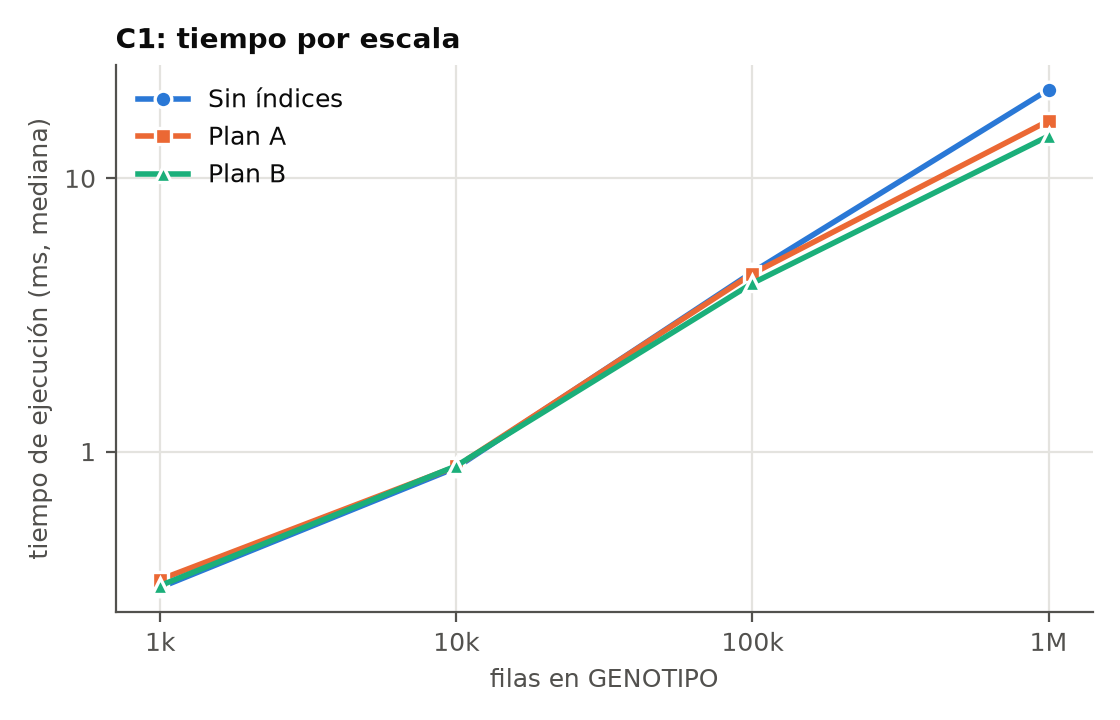
\includegraphics[width=0.72\textwidth]{fig/C1.png}
\caption{C1: tiempo de ejecución por escenario.}
\end{figure}

Es la consulta más rápida en todos los escenarios porque filtra por un solo donante. Hasta 100k los tres casos empatan. En 1M el plan A baja de 21.1 a 16.2 ms y el plan B a 14.3 ms (1.5$\times$): el índice parcial ocupa 0.36 MB frente a 1.68 MB del índice completo, y como solo contiene anotaciones patogénicas el filtro de significancia ya viene resuelto. Sin índices la consulta ya era rápida gracias a que la llave primaria de \texttt{genotipo} empieza por \texttt{id\_\allowbreak{}muestra}.

\subsubsection*{C2. Portadores por gen}

\begin{figure}[H]
\centering
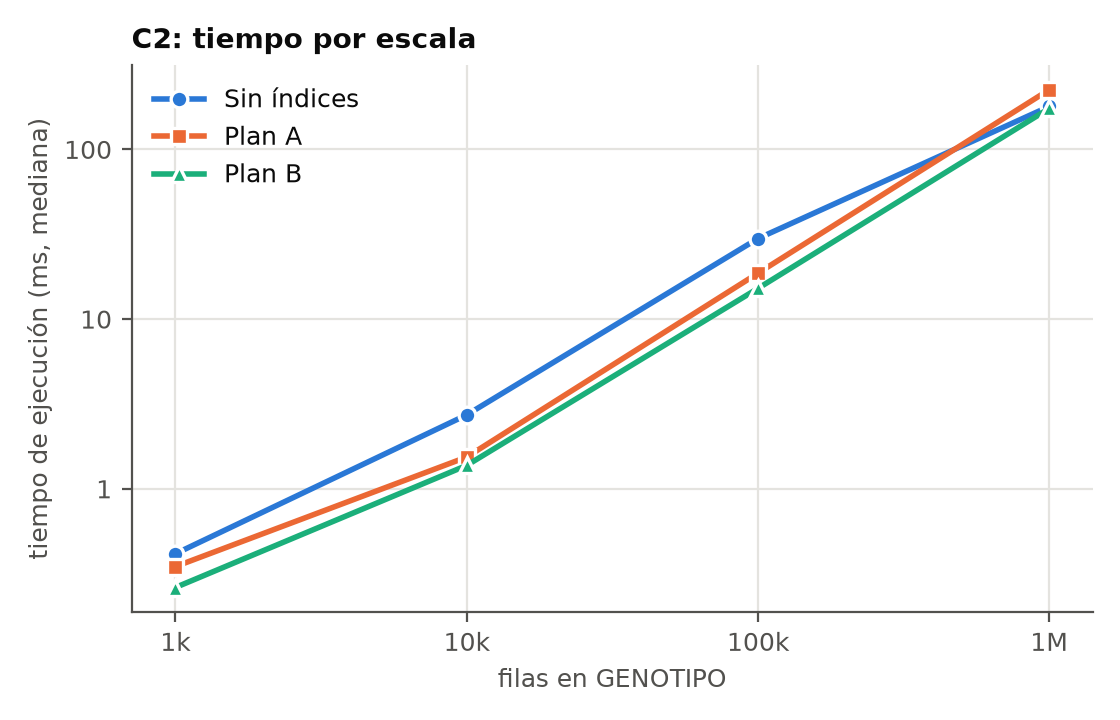
\includegraphics[width=0.72\textwidth]{fig/C2.png}
\caption{C2: tiempo de ejecución por escenario.}
\end{figure}

Es el caso más interesante. En 10k y 100k los dos planes ayudan (en 100k: 29.8 ms sin índices, 18.6 con A y 15.2 con B). Pero en 1M el plan A es \textbf{más lento} que no tener índices (225 frente a 179 ms). El plan muestra por qué: el planificador entra a \texttt{genotipo} por el índice una vez por cada variante patogénica, y cada fila encontrada obliga a leer una página distinta de la tabla. Cerca del 5.8\,\% de los genotipos tiene una variante patogénica (unas 58\,000 filas en 1M); a ese volumen, leer la tabla completa en orden y en paralelo cuesta menos que tantos accesos aleatorios. El plan B evita esas visitas a la tabla con un \textit{Index Only Scan} y queda empatado con la lectura completa (175 ms).

\subsubsection*{C3. Variantes enriquecidas en la cohorte}

\begin{figure}[H]
\centering
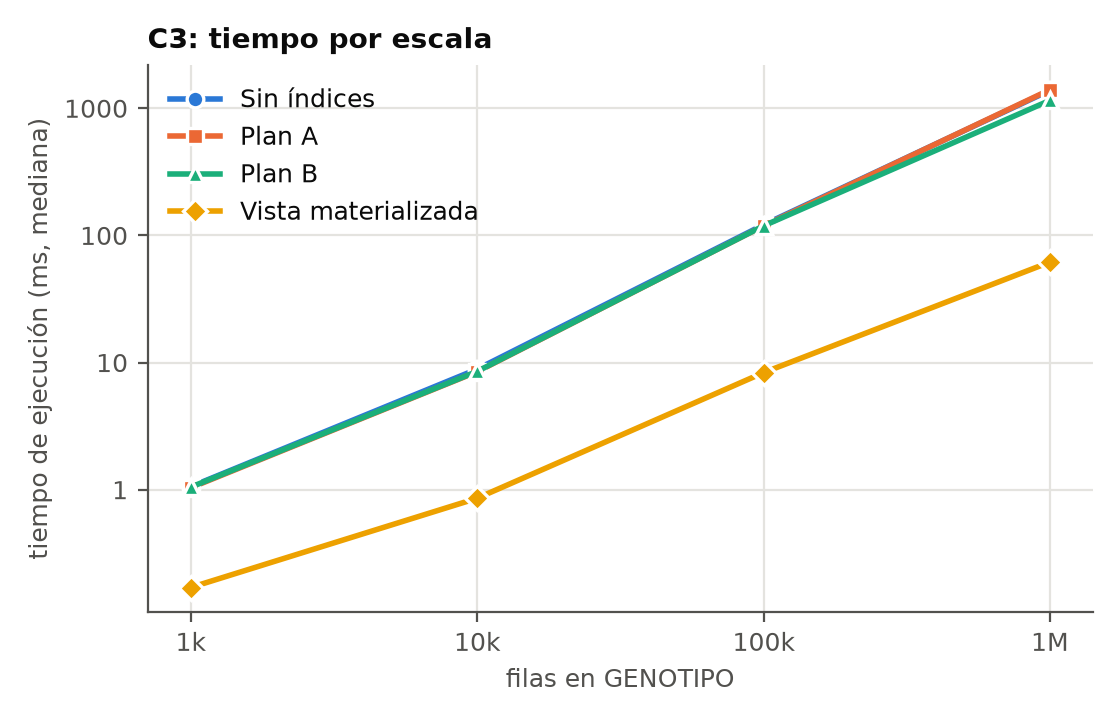
\includegraphics[width=0.72\textwidth]{fig/C3.png}
\caption{C3: tiempo de ejecución por escenario.}
\end{figure}

Ningún índice cambia mucho el tiempo, como se esperaba: la consulta lee el millón de filas igual. Con el plan A el planificador ni siquiera usa el índice (sigue haciendo \textit{Seq Scan}). El plan B sí se usa y baja de 1\,384 a 1\,154 ms (1.2$\times$) porque recorre el índice ya ordenado y se ahorra el ordenamiento del \texttt{GROUP BY}. La mejora real viene de la vista materializada: la misma respuesta en 61.7 ms, 22 veces más rápido. Su costo es que hay que refrescarla (1\,248 ms en 1M) y que entre refrescos sus datos quedan desactualizados.

\subsubsection*{C5. Consulta por región genómica}

\begin{figure}[H]
\centering
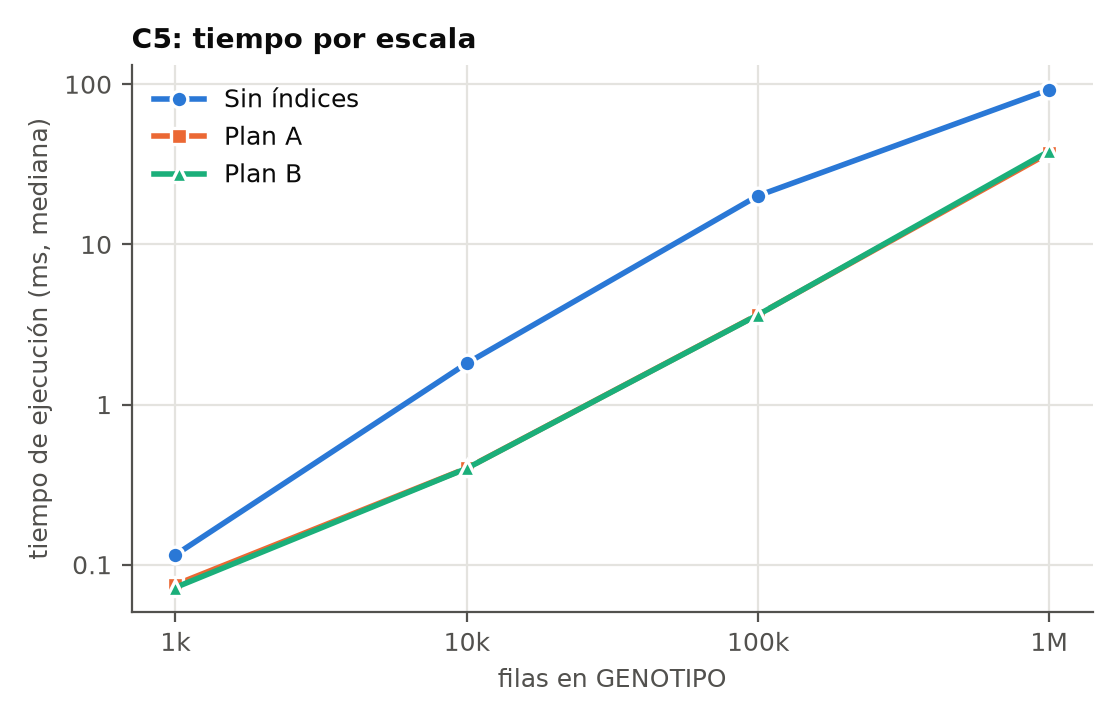
\includegraphics[width=0.72\textwidth]{fig/C5.png}
\caption{C5: tiempo de ejecución por escenario.}
\end{figure}

El índice sobre \texttt{genotipo(id\_\allowbreak{}variante)} es el que importa: en 1M el tiempo baja de 92.5 a 37.3 ms (2.5$\times$) y en 100k de 20.1 a 3.64 ms (5.5$\times$). El índice hash y el B-tree dan prácticamente el mismo tiempo, pero el B-tree además sirve para rangos y ordenamiento, así que no hay razón para preferir el hash. El índice de región \texttt{ix\_\allowbreak{}var\_\allowbreak{}region} resultó \textbf{redundante}: incluso sin él, el planificador ya usaba el índice del \texttt{UNIQUE} \texttt{(id\_\allowbreak{}cromosoma, posicion, alelo\_\allowbreak{}ref, alelo\_\allowbreak{}alt)} de la llave natural, que empieza por las mismas dos columnas. Por eso no quedó entre los índices finales.

\subsubsection*{C6. Concordancia técnica entre corridas}

\begin{figure}[H]
\centering
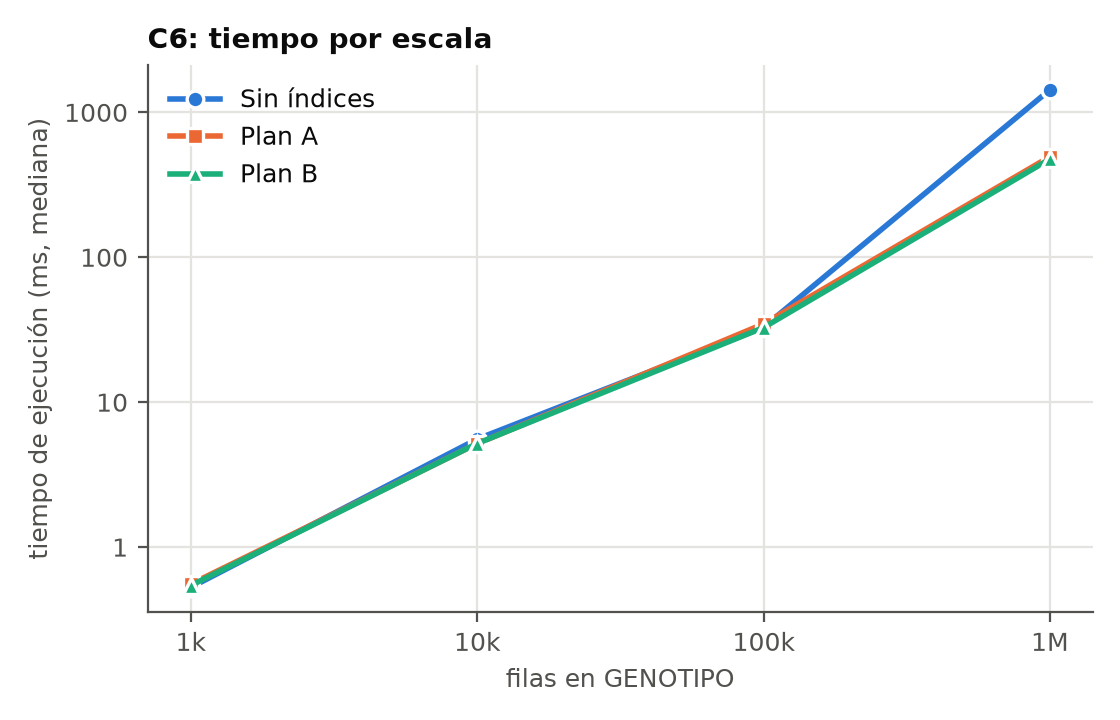
\includegraphics[width=0.72\textwidth]{fig/C6.png}
\caption{C6: tiempo de ejecución por escenario.}
\end{figure}

Hasta 100k los índices no cambian nada, pero en 1M es la consulta que más gana: de 1\,434 a 495 ms con el plan A (2.9$\times$) y 477 ms con el B. Sin índices hay que construir una tabla hash con el millón de genotipos para el self-join; con el índice, cada genotipo de una muestra re-secuenciada busca directamente su pareja. El orden de las columnas no importa aquí porque el join usa las dos con igualdad. Una prueba adicional con \texttt{INCLUDE (id\_\allowbreak{}corrida, genotipo)} permitió un \textit{Index Only Scan} y bajó a unos 436 ms.

\begin{figure}[H]
\centering
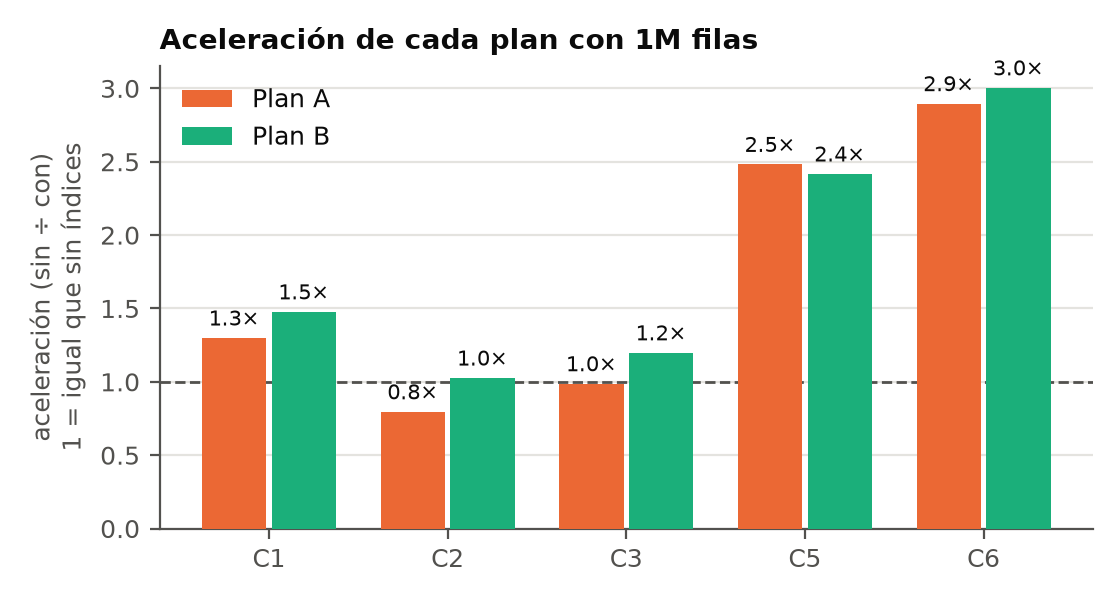
\includegraphics[width=0.72\textwidth]{fig/aceleracion_1M.png}
\caption{Aceleración de cada plan con 1M de genotipos. Una barra bajo 1 significa que el plan empeora la consulta.}
\end{figure}

\subsubsection*{Costo de los índices en las actualizaciones}

Cada índice hace más rápida la lectura pero más lenta la escritura, porque cada \texttt{INSERT} y cada
\texttt{UPDATE} que toca una columna indexada debe actualizar también el índice. Se compararon los tiempos sin
índices y con los índices finales:

\begin{figure}[H]
\centering
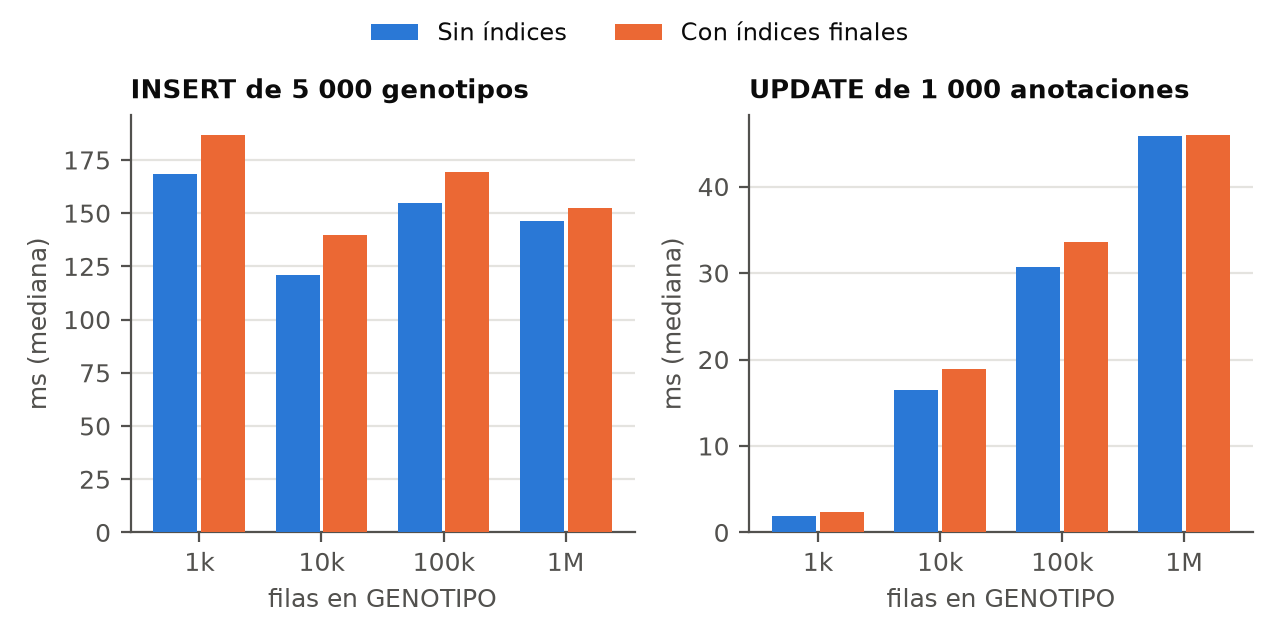
\includegraphics[width=0.85\textwidth]{fig/actualizaciones.png}
\caption{Costo de las actualizaciones sin índices y con los índices finales.}
\end{figure}

\begin{table}[H]
\centering\small
\begin{tabular}{@{}llrrrr@{}}
\toprule
Operación & Índices & 1k & 10k & 100k & 1M \\
\midrule
INSERT de 5\,000 genotipos & sin índices & 168 & 121 & 155 & 146 \\
INSERT de 5\,000 genotipos & con índices finales & 187 & 140 & 169 & 153 \\
\multicolumn{2}{r}{\textit{sobrecosto en 1M}} & & & & +4\,\% \\
\midrule
UPDATE de 1\,000 anotaciones & sin índices & 1.86 & 16.4 & 30.7 & 45.8 \\
UPDATE de 1\,000 anotaciones & con índices finales & 2.32 & 18.9 & 33.6 & 46.0 \\
\multicolumn{2}{r}{\textit{sobrecosto en 1M}} & & & & +0\,\% \\
\bottomrule
\end{tabular}
\caption{Tiempo de las actualizaciones (ms, mediana de 7). En 1k hay solo 76 anotaciones, por eso el UPDATE toca menos filas.}
\end{table}

Con los índices finales, insertar 5\,000 genotipos en 1M pasa de 146 a 153 ms. El
sobrecosto es pequeño porque la mayor parte del tiempo de esa inserción se va en verificar la llave primaria y
la llave foránea compuesta de cada fila, que existen con o sin los índices del experimento. En el \texttt{UPDATE} de
anotaciones la diferencia es casi nula: cambiar \texttt{significancia} solo obliga a mantener el índice parcial,
que es diminuto. El costo que sí crece es el espacio:

\begin{table}[H]
\centering\small
\begin{tabular}{@{}lr@{}}
\toprule
Índice & Tamaño en 1M (MB) \\
\midrule
\texttt{ix\_\allowbreak{}gen\_\allowbreak{}mue\_\allowbreak{}var} & 51.71 \\
\texttt{ix\_\allowbreak{}gen\_\allowbreak{}var\_\allowbreak{}mue} & 51.65 \\
\texttt{ix\_\allowbreak{}anot\_\allowbreak{}variante} & 1.68 \\
\texttt{ix\_\allowbreak{}anot\_\allowbreak{}patog} & 0.36 \\
\texttt{ix\_\allowbreak{}muestra\_\allowbreak{}donante} & 0.06 \\
\midrule
Tabla \texttt{genotipo} sin índices (heap) & 91.1 \\
Tabla \texttt{genotipo} con todos sus índices & 260.0 \\
\bottomrule
\end{tabular}
\caption{Tamaño de los índices finales con 1M de genotipos.}
\end{table}

Los dos índices cubrientes de \texttt{genotipo} ocupan, juntos, más que la propia tabla. En la carga semanal de
una corrida grande (millones de filas por \texttt{COPY}) conviene borrar esos índices antes de la carga y
recrearlos después: crearlos todos tomó 2.1 s en 1M, menos que mantenerlos fila por fila.

\subsection{Análisis y discusión}

\begin{enumerate}
  \item \textbf{Con pocos datos los índices no importan.} En 1k y 10k todas las consultas tardan menos de
        10 ms con o sin índices: las tablas caben en pocas páginas y leerlas completas es tan rápido como usar un
        índice. Las diferencias aparecen desde 100k y se hacen claras en 1M.
  \item \textbf{El índice ayuda cuando la consulta es selectiva.} C1 (un donante), C5 (una región) y C6 (solo las
        muestras re-secuenciadas, cerca del 10\,\%) leen una fracción pequeña de \texttt{genotipo}, y ahí los
        índices dan entre 1.5 y 3 veces de mejora en 1M. C3 lee toda la tabla y ningún índice la salva.
  \item \textbf{Un índice puede empeorar una consulta.} En C2 el plan A hizo la consulta 25\,\% más lenta en 1M,
        porque el planificador prefirió muchos accesos aleatorios a la tabla en vez de una lectura secuencial en
        paralelo. Los índices cubrientes (\texttt{INCLUDE}) evitan ese problema porque no visitan la tabla.
  \item \textbf{Para agregaciones de toda la tabla, la solución es precalcular.} La vista materializada hace que C3
        sea 22 veces más rápida. Como los genotipos se cargan una vez por semana
        (Sección~1.5.4), basta con hacer \texttt{REFRESH MATERIALIZED VIEW} después de cada carga, lo que en 1M
        tomó 1.2 s.
  \item \textbf{Las restricciones ya crean índices.} La llave primaria de \texttt{genotipo} sirve para C1 y el
        \texttt{UNIQUE} de la llave natural de \texttt{variante} hace innecesario el índice de región de C5. Antes de
        crear un índice hay que revisar si una restricción ya lo creó.
  \item \textbf{B-tree frente a hash.} En C5 dieron el mismo tiempo. El B-tree sirve también para rangos y para
        \texttt{ORDER BY}; el hash solo para igualdad. No hay motivo para usar hash en este caso.
  \item \textbf{Todas las consultas cumplen los tiempos esperados del Hito~1.} Con los índices finales y 1M de
        genotipos: C1 tarda 14.3 ms y C5 37.3 ms (se pedía menos de 1 s); C2, C3 y C6 tardan
        menos de 1.5 s (se pedía menos de 10 s).
\end{enumerate}

\paragraph{Índices finales.} Con estos resultados quedan en la base de datos (\texttt{08\_\allowbreak{}indices.sql}):

\begin{lstlisting}[language=SQL]
CREATE INDEX IF NOT EXISTS ix_muestra_donante ON muestra(id_donante);
CREATE INDEX IF NOT EXISTS ix_anot_patog ON anotacion_clinica(id_variante) WHERE significancia IN ('PATOGENICA','PROBABLEMENTE_PATOGENICA');
CREATE INDEX IF NOT EXISTS ix_anot_variante ON anotacion_clinica(id_variante);
CREATE INDEX IF NOT EXISTS ix_gen_var_mue ON genotipo(id_variante, id_muestra) INCLUDE (genotipo);
CREATE INDEX IF NOT EXISTS ix_gen_mue_var ON genotipo(id_muestra, id_variante) INCLUDE (genotipo);
\end{lstlisting}

\texttt{ix\_\allowbreak{}anot\_\allowbreak{}variante} se mantiene aunque C1 prefiere el índice parcial, porque \texttt{anotacion\_\allowbreak{}clinica.id\_\allowbreak{}variante}
es una llave foránea con \texttt{ON DELETE CASCADE} y las búsquedas de C7 piden todas las anotaciones de una variante.

\subsection{Pregunta adicional: ¿qué pasa con más de 1M de registros?}\label{sec:extra}

El Hito~1 estimó unos $10^8$ genotipos (6.5 GB sin índices) para los primeros años del CGA con exomas, y decenas de
miles de millones si se pasara a genomas completos. Según las mediciones:

\begin{itemize}
  \item Las consultas selectivas que usan índices (C1, C5) crecen mucho más lento que los datos: el B-tree
        tiene pocos niveles (crece con el logaritmo del número de filas), así que en $10^8$ filas seguirían en el
        orden de decenas o cientos de milisegundos.
  \item Las que leen toda la tabla (C3 y, en parte, C2 y C6) crecen en proporción a los datos: en las figuras su
        pendiente es cercana a 1. Pasar de $10^6$ a $10^8$ filas multiplicaría su tiempo por cerca de 100; C3 tardaría
        un par de minutos. Para ellas hacen falta vistas materializadas o tablas de resumen que se actualicen
        con cada carga.
  \item Al crecer, la tabla y sus índices dejan de caber en memoria y cada acceso aleatorio se vuelve una lectura
        de disco. Hay que subir \texttt{shared\_\allowbreak{}buffers} y \texttt{work\_\allowbreak{}mem} y usar discos SSD.
\end{itemize}

\textbf{¿Basta con la arquitectura cliente--servidor?} Para $10^8$ filas sí: un solo servidor PostgreSQL bien
configurado, con \textbf{particionamiento} de \texttt{genotipo} (por ejemplo por cromosoma o por rango de
\texttt{id\_\allowbreak{}corrida}) para que cada consulta solo lea las particiones que necesita, y con índices por partición.
Para decenas de miles de millones de filas (genomas completos) un solo servidor ya no alcanza ni en disco ni en
tiempo de carga, y hay que distribuir los datos: réplicas de solo lectura para repartir las consultas y
\textit{sharding} de \texttt{genotipo} por cromosoma o por donante entre varios nodos (por ejemplo con Citus, que
extiende PostgreSQL), o un almacén columnar para las agregaciones poblacionales como C3.

\section{Conclusiones}

\begin{itemize}
  \item Se implementó en PostgreSQL el modelo del Hito~1 con todas sus reglas semánticas: las que caben en una tabla
        como restricciones declarativas y las demás como nueve triggers, y se comprobó con 12 pruebas que se cumplen.
  \item Una llave foránea compuesta resolvió RS19 sin código, y un trigger diferido resolvió la especialización
        total, que no se puede expresar con un \texttt{CHECK}.
  \item Los índices no siempre ayudan: sirven cuando la consulta es selectiva y la tabla es grande (hasta 3 veces
        más rápido en C6 con 1M de filas), no sirven cuando la consulta lee toda la tabla (C3) y pueden empeorarla
        cuando obligan a muchos accesos aleatorios (C2, plan A).
  \item Para las agregaciones de toda la cohorte, una vista materializada refrescada después de cada carga
        semanal es mucho más efectiva que cualquier índice.
  \item El costo de mantener los índices finales en las actualizaciones fue bajo, pero ocupan más espacio que la
        propia tabla de hechos.
  \item Con 1M de genotipos todas las consultas cumplen los tiempos de respuesta esperados.
\end{itemize}


\section{Anexos}

\subsection{Video del experimento}

Video del experimento con 1M de registros, con y sin índices: \textbf{[enlace al video]}.

En el video se restaura \texttt{dumps/genvar\_\allowbreak{}1000000.dump}, se ejecutan las consultas de \texttt{07\_\allowbreak{}consultas.sql}
sin índices con \texttt{\textbackslash timing on}, se crean los índices con \texttt{08\_\allowbreak{}indices.sql} y se vuelven a
ejecutar las mismas consultas.

\subsection{MVP web}

Como punto extra se desarrolló una aplicación web en Python (Flask) conectada directamente a la base de datos
PostgreSQL (carpeta \texttt{web/}). Permite:

\begin{itemize}
  \item Ejecutar las consultas C1 a C8 con sus parámetros y ver el resultado, el tiempo, el SQL y el plan de ejecución.
        Las cinco consultas del experimento usan el mismo SQL de la Sección~5.1.2.
  \item Ver la ficha de un donante con sus muestras y su reporte clínico (\texttt{fn\_\allowbreak{}reporte\_\allowbreak{}clinico}).
  \item Registrar donantes y muestras, reclasificar anotaciones y revocar consentimientos con los procedimientos
        almacenados. Cuando una operación viola una regla, la aplicación muestra el error que lanza el trigger
        (por ejemplo, T3 al registrar una muestra de un donante sin consentimiento).
  \item Borrar y crear los índices finales y comparar los tiempos de las cinco consultas del experimento.
  \item Actuar como cada tipo de usuario (\texttt{SET ROLE}) para comprobar los permisos de la Sección~4.4.
\end{itemize}

Se ejecuta con \texttt{pip install -r web/requirements.txt} y \texttt{python web/app.py}, y se abre en
\texttt{http://localhost:5000}.

\begin{figure}[H]
\centering
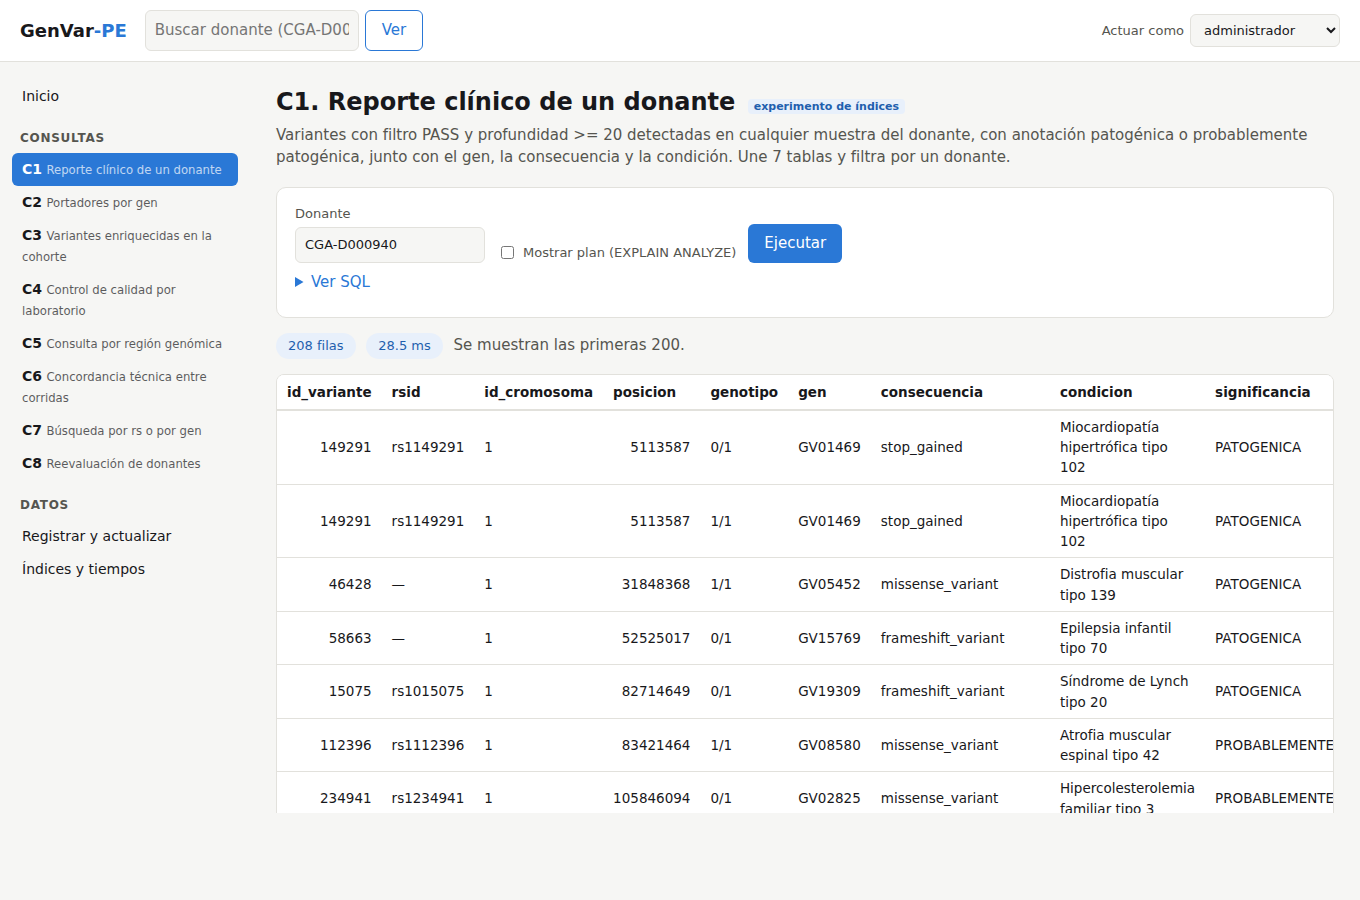
\includegraphics[width=0.9\textwidth]{fig/web_consulta.png}
\caption{MVP web: ejecución de la consulta C1 con 1M de genotipos.}
\end{figure}

\begin{figure}[H]
\centering
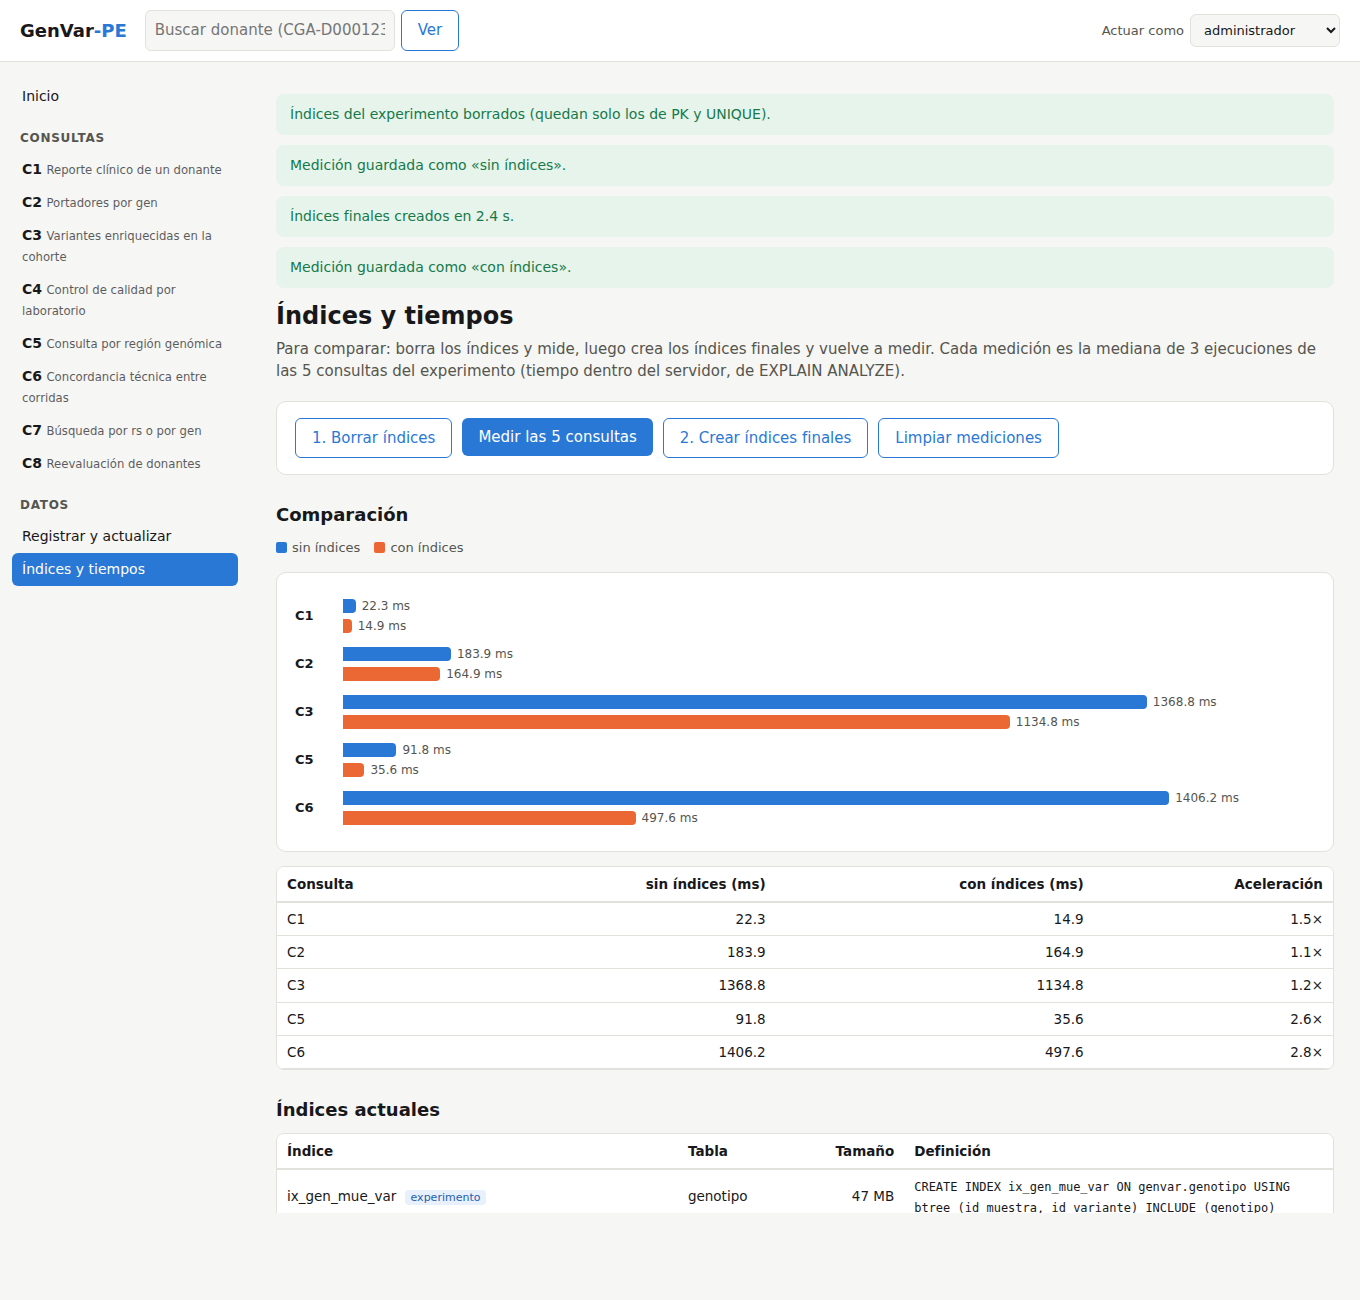
\includegraphics[width=0.9\textwidth]{fig/web_indices.png}
\caption{MVP web: comparación de tiempos sin índices y con los índices finales.}
\end{figure}

\subsection{Archivos entregados}

\begin{table}[H]
\centering\small
\begin{tabular}{@{}l>{\raggedright\arraybackslash}p{9.5cm}@{}}
\toprule
Ruta & Contenido \\
\midrule
\texttt{sql/} & Scripts 01 a 09 (Sección 4 y 5) \\
\texttt{dumps/} & Los cuatro dumps: \texttt{genvar\_\allowbreak{}1000.dump}, \texttt{genvar\_\allowbreak{}10000.dump}, \texttt{genvar\_\allowbreak{}100000.dump}, \texttt{genvar\_\allowbreak{}1000000.dump} \\
\texttt{exp/consultas.py} & Consultas y planes de índices (fuente única) \\
\texttt{exp/experimento.py} & Script que genera los escenarios y mide los tiempos \\
\texttt{exp/resultados.json} & Todas las mediciones (las 7 repeticiones, planes usados y filas) \\
\texttt{exp/graficos.py} & Genera las figuras de la Sección 5.6 \\
\texttt{exp/salida\_\allowbreak{}pruebas.txt} & Salida de \texttt{09\_\allowbreak{}pruebas.sql} \\
\texttt{web/} & MVP web (Flask): \texttt{app.py}, plantillas y \texttt{LEEME.md} con las instrucciones \\
\bottomrule
\end{tabular}
\caption{Contenido del repositorio del proyecto.}
\end{table}

\subsection{Cómo reproducir el experimento}

\begin{lstlisting}[language=bash]
createdb genvar
for f in 01_esquema 02_vistas 03_procedimientos 04_triggers 05_roles; do
  psql -d genvar -f sql/$f.sql
done
pip install psycopg2-binary matplotlib
python3 exp/experimento.py --reps 7     # genera los 4 escenarios, los dumps y resultados.json
python3 exp/graficos.py                 # genera fig/*.png
psql -d genvar -f sql/08_indices.sql    # deja los índices finales
psql -d genvar -f sql/09_pruebas.sql    # pruebas de triggers y procedimientos
\end{lstlisting}

\end{document}
